\documentclass[12pt,a4paper,oneside]{report}

\usepackage[a4paper,margin=1in]{geometry}
\usepackage[T1]{fontenc}
\usepackage[utf8]{inputenc}
\usepackage{lmodern}
\usepackage{graphicx}
\usepackage{booktabs}
\usepackage{longtable}
\usepackage{array}
\usepackage{tabularx}
\usepackage{enumitem}
\usepackage{setspace}
\usepackage{titlesec}
\usepackage{xcolor}
\usepackage{hyperref}
\usepackage{listings}
\usepackage{caption}
\usepackage{float}
\usepackage{amsmath}
\usepackage{amssymb}
\usepackage{fancyhdr}
\usepackage{url}
\usepackage{tikz}
\usetikzlibrary{arrows.meta}
\usepackage{colortbl}

\definecolor{mtunavy}{HTML}{1B2A4A}
\definecolor{mtuamber}{HTML}{F5C518}
\definecolor{codebg}{HTML}{F6F8FA}

\hypersetup{
  colorlinks=true,
  linkcolor=mtunavy,
  citecolor=mtunavy,
  urlcolor=mtunavy,
  plainpages=false,
  hypertexnames=false,
  pdftitle={ELA: English Language Assistant},
  pdfauthor={Vladyslav Rastvorov}
}

\lstdefinestyle{jsonstyle}{
  basicstyle=\ttfamily\small,
  backgroundcolor=\color{codebg},
  frame=single,
  breaklines=true,
  columns=fullflexible,
  keepspaces=true,
  showstringspaces=false
}

\setlength{\headheight}{15pt}
\pagestyle{fancy}
\fancyhf{}
\fancyhead[R]{\thepage}
\fancyhead[L]{ELA: English Language Assistant}

\titleformat{\chapter}[display]
  {\normalfont\bfseries\color{mtunavy}}
  {\filleft\Huge\chaptername\ \thechapter}
  {1ex}
  {\titlerule\vspace{1ex}\filright\Huge}

\setlist[itemize]{topsep=4pt,itemsep=3pt}
\setlist[enumerate]{topsep=4pt,itemsep=3pt}
\onehalfspacing

\begin{document}
\hypersetup{pageanchor=false}

\begin{titlepage}
  \centering
  \vspace*{1.5cm}
  {\color{mtunavy}\rule{\textwidth}{1.2pt}\par}
  \vspace{0.6cm}
  {\Huge\bfseries ELA: English Language Assistant\par}
  \vspace{0.4cm}
  {\Large Recursive Linguistic Elements, Multimodal Processing, and Explainable Support for Authentic English Input\par}
  \vspace{0.8cm}
  {\color{mtuamber}\rule{0.72\textwidth}{1.2pt}\par}
  \vspace{1.1cm}

  \includegraphics[width=0.22\textwidth]{../Figures/MTUCREST.jpg}\par
  \vspace{1.1cm}

  {\Large Vladyslav Rastvorov\par}
  \vspace{0.2cm}
  {\large R00274535\par}
  \vspace{1.1cm}

  {\large This thesis has been submitted in partial fulfillment for the degree of\par}
  \vspace{0.2cm}
  {\Large\bfseries Bachelor of Science (Honours) in Computer Systems\par}
  \vspace{0.9cm}

  {\large Faculty of Engineering and Science\par}
  {\large Department of Computer Science\par}
  {\large Munster Technological University Cork\par}
  \vspace{1cm}

  \begin{tabular}{>{\bfseries}p{4.2cm}p{8.5cm}}
    Research Supervisor: & Dr. Alex Vakaloudis \\
    Implementation Supervisor: & Dr. Nasir Ahmad \\
    Academic Year: & 2024--2025 \\
    Submission Date: & April 2026 \\
    Live system: & \url{https://el-a.uk} \\
    Source code: & \url{https://github.com/welsol21/FYP_LLM} \\
  \end{tabular}

  \vfill
  {\color{mtunavy}\rule{\textwidth}{1.2pt}\par}
\end{titlepage}

\pagenumbering{roman}

\chapter*{Declaration of Authorship}
This report, \emph{ELA: English Language Assistant}, is submitted in partial fulfillment of the requirements for the degree of Bachelor of Science (Honours) in Computer Systems at Munster Technological University Cork. I, Vladyslav Rastvorov, declare that the work presented in this thesis is substantially my own except where explicitly stated.

\begin{itemize}
  \item This work was carried out wholly or mainly while in candidature for the above degree at Munster Technological University Cork.
  \item Where any part of this thesis has previously been submitted for another qualification, this has been clearly stated.
  \item Where I have consulted the published work of others, this is always clearly attributed.
  \item Where I have quoted from the work of others, the source is always given.
  \item I have acknowledged all main sources of help.
  \item Where the thesis is based on work carried out jointly with others, I have made clear what was done by others and what I contributed myself.
\end{itemize}

\vspace{1.4cm}
\noindent Signed:\ \rule{7cm}{0.4pt}

\vspace{0.8cm}
\noindent Date:\ \rule{4cm}{0.4pt}

\chapter*{Abstract}
This thesis presents the continued development of the English Language Assistant (ELA), a full-stack language learning system designed to make authentic English input more accessible without simplifying or rewriting the source material. ELA ingests text, audio, and video, then transforms the input into a hierarchical contract of \emph{Recursive Linguistic Elements} (RLE), where each sentence is represented as a structured tree of sentence, phrase, and word nodes enriched with grammatical, pedagogical, and bilingual metadata.

The project implements two interconnected approaches. The first is focused on practical support for learners of English, especially users with intermediate and advanced levels of proficiency. For this purpose, a Progressive Web Application (PWA) was developed, bringing together tools for the analysis of authentic English material, the visualization of linguistic relations within a sentence, and the creation of custom learning materials in text, audio, and video form. Particular attention was given to usability: the interface was designed to be intuitive, visually clear, and convenient for everyday use on mobile devices. Within this practical direction, the system was intended not simply to help users read or listen to English, but to support deeper immersion into its grammatical and linguistic structures, including work with bilingual materials and learning based on real, unsimplified content.

The second approach belongs to the research dimension of the project and is aimed at the scientific analysis of relationships between linguistic and grammatical constructions in English. Its purpose is to treat language not as an unlimited collection of isolated examples, but as a system in which a finite number of recurring structural patterns can be identified. For this, the project uses the RLE contract, where RLE stands for Recursive Linguistic Elements, a formal representation developed specifically for this line of research in the earlier research phase of the project. Through this model, a sentence can be described as an organized system of interrelated elements, making it possible not only to analyse individual linguistic phenomena, but also to investigate broader regularities that underlie English grammar.

This idea received empirical support in a separate experiment on the task of selecting a pedagogical note on the basis of the structure of an English sentence. The results showed that when the input representation preserves the recursive structure of the sentence in the form of an RLE contract, note selection improves even when the classifier itself remains comparatively simple. This is important because it supports the central hypothesis of the project: the grammatical structure of language, and not only its lexical content, can serve as a learnable and predictive basis for subsequent interpretation.

The final result of this work is a fully functional and reproducible pipeline which takes an English input sentence, constructs a hierarchical JSON representation according to the project's RLE contract, and enriches it with linguistic notes. These notes are, in turn, produced on the basis of transformer-classifier inference and then refined for more natural phrasing by a T5-small language model adapted to this task. The classifier itself is also trained not in a single step but in several consecutive stages, in which the structural representation of the sentence, note classification, and the subsequent generation of its final form are combined into one connected system. In this way, the work presents ELA both as an operational system and as an ongoing research programme.

\chapter*{Acknowledgements}
I would like to thank my supervisors, Dr. Alex Vakaloudis and Dr. Nasir Ahmad, for their guidance across both the research and implementation dimensions of this project. I am also grateful to my family for their continuing support throughout the development of ELA, and to Munster Technological University Cork for providing the environment in which this work could take shape.

\tableofcontents
\listoffigures
\listoftables

\chapter*{List of Abbreviations}
\begin{longtable}{>{\bfseries}p{3cm}p{10cm}}
ASR & Automatic Speech Recognition \\
CALL & Computer-Assisted Language Learning \\
CEFR & Common European Framework of Reference for Languages \\
FR & Functional Requirement \\
IPA & International Phonetic Alphabet \\
LLM & Large Language Model \\
ML & Machine Learning \\
NFR & Non-Functional Requirement \\
NLP & Natural Language Processing \\
POS & Part of Speech \\
PWA & Progressive Web Application \\
RLE & Recursive Linguistic Elements \\
TAM & Tense, Aspect, and Mood \\
WER & Word Error Rate \\
\end{longtable}

\clearpage
\hypersetup{pageanchor=true}
\pagenumbering{arabic}

\chapter{Introduction}
\section{Motivation}
Most digital language-learning systems lower difficulty by reducing or simplifying the source material. This makes early progress easier, but it also distances the learner from real English as it appears in speech, media, and written communication. Authentic input is richer, more motivating, and more representative of actual language use, but it is also harder to process without support. The central motivation of ELA is therefore not to simplify authentic English, but to make it explainable.

\section{Problem Statement}
Many learners of English encounter serious difficulties when working with authentic materials such as articles, lectures, podcasts, and audio or video content. Such materials contain dense vocabulary, complex grammatical constructions, idiomatic expressions, and natural speech patterns that make comprehension difficult even for learners at intermediate and advanced levels. Most existing systems address this problem either by simplifying the content, by training isolated skills, or by providing explanations that are too general and too opaque to reflect the real internal structure of the language. As a result, a clear gap remains between classroom English and the English of real communication. ELA takes a different approach: instead of altering the source material, it makes authentic input more accessible through explainable decomposition into interpretable linguistic units and by adding structured support on top of the original text, audio, or video.

This also defines the scope of the present thesis. Its scope includes the implemented system architecture, the linguistic contract, the multimodal runtime path, the frontend visualization layer, and the experimental line concerned with structural abstraction in the generation of pedagogical notes. Outside the scope of this thesis are large-scale classroom deployment and strong claims about measurable learning gains based on user studies. This boundary is intentional, because the thesis treats ELA primarily as a research-engineering system rather than as a fully validated educational product.

\section{Research Questions}
This thesis is structured around three research questions:
\begin{enumerate}
  \item How can authentic text, audio, and video material be transformed into structured representations suitable for pedagogical interpretation without simplifying the original content?
  \item What model of representation best captures the relationships between the levels of sentence, phrase, and word while remaining sufficiently stable for validation, storage, visualization, and further computational processing?
  \item To what extent can structural abstraction, particularly in the form of templates and placeholders, improve the system's ability to generalize when generating pedagogical notes for new language examples?
\end{enumerate}

\section{Objectives}
The ELA implementation phase is organized around the following goals:
\begin{enumerate}
  \item Construct a multimodal processing pipeline that takes in text, audio, and video and converts them into structured sentence-level representations.
  \item Formalize a hierarchical contract capable of carrying grammatical, pedagogical, and bilingual metadata in a stable and validated form.
  \item Provide a learner-facing application that exposes linguistic structure through an interactive visualizer, export flow, and media-oriented workflow.
  \item Explore whether abstract structural templates support stronger note-generation generalization than raw lexical notation.
\end{enumerate}

\section{Contributions}
These contributions were the following:
\begin{itemize}
  \item an improved implementation of ELA as a complete-stack system rather than a prototype, deployed at \url{https://el-a.uk} and available as open-source at~[16];
  \item the formalization and operationalization of the RLE contract as the core data interface between backend, storage, and frontend;
  \item a rules-first linguistic pipeline that integrates parsing, phrase construction, TAM enrichment, CEFR estimation, translation, phonetic support, and pedagogical notes;
  \item a research analysis of the placeholder strategy for note generation through the context--pattern duality;
  \item a detailed evaluation of the current system covering implemented capabilities, empirical evidence, and unresolved limitations.
\end{itemize}

Taken together, these results allow the thesis to be understood both as a description of an implemented system and as an investigation of the principles of structural representation in language. The practical contribution of the work lies in the creation of a functioning ELA stack which combines the processing of authentic English material, its structural analysis, and user-facing tools for working with the results of that analysis. The research contribution lies in the further confirmation of the central idea of ELA: each sentence can be decomposed into Recursive Linguistic Elements, that is, into the levels of sentence, phrase, and word, and each such element can be described through abstract grammatical attributes rather than through specific words. This, in turn, allows the system to identify stable structural patterns and to use them when working with new language examples of the same grammatical form.

\section{Thesis Structure}
The remainder of the thesis is organized as follows. Chapter 2 reviews the theoretical and applied fields on which ELA draws, including Computer-Assisted Language Learning, authentic materials, NLP-based analysis, CEFR, generative models, and multimodal processing. Chapter 3 connects the current work to the earlier research phase of the project and shows how ELA developed from a conceptual prototype into an implemented system. Chapter 4 describes the RLE data model and explains the contract that underlies the representation of linguistic structure. Chapter 5 is devoted to the idea of context--pattern duality and to the role of structural abstraction in the generation of pedagogical notes. Chapter 6 presents the architecture and implementation of the system, including the backend, runtime, frontend, and multimodal components. Chapter 7 examines dataset and corpus engineering. Chapter 8 evaluates the system and analyses the results obtained. Chapter 9 discusses the limitations of the work and possible directions for further development. Chapter 10 concludes the thesis. After the main body, additional chapters provide repository-based evidence sources, an index of evaluation artefacts, and examples of templates used in the pipeline.

\chapter{Background and Related Work}
\section{Computer-Assisted Language Learning}
Computer-Assisted Language Learning (CALL) provides the pedagogical background of ELA. Contemporary systems in this area include adaptation, learner modelling, multimodal content, and mobile forms of delivery. The present project develops in this direction by proposing an extension of existing learning tools and methodologies through the active inclusion of authentic language content in the learning process. At the same time, the emphasis is placed not only on the technological side of the system, but also on learner autonomy and on gradual, guided support while working with the material.

Within this approach, software should not simply replace the learner's own analysis. On the contrary, it should externalize part of that analysis in a form that the learner can see, inspect, and explore. This is especially important in independent learning scenarios, where the system should function not only as an exercise tool, but also as a structured explanatory assistant, or, as it is called in this thesis, an English Learning Assistant (ELA).

\section{Authentic Materials and Cognitive Support}
Authentic materials occupy an important place in language learning because they preserve the vocabulary, grammatical constructions, pragmatics, and stylistic features of real communication. It is through such materials that the learner encounters features of language that are rarely fully present in artificially simplified textbook examples: natural tense shifts, fixed expressions, characteristic linking phrases, and the way speakers actually express their thoughts. At the same time, the very qualities that make authentic material valuable also make it more difficult to process.

This creates a central methodological tension. If authentic material is simplified too aggressively, it loses a significant part of its educational value. If it is left in its original form without additional support, it may become too difficult even for a motivated learner. ELA addresses precisely this problem: the system does not rewrite the original material, but instead adds a layer of structured and explainable support to it. In this sense, the project stands at the intersection of authenticity, pedagogical support, and transparency, since it aims to preserve the original utterance while making its internal structure accessible for study.

\section{NLP Parsing and Structured Analysis}
ELA uses modern NLP tools to extract syntactic and morphological information from English text, including tokenization, lemmatization, part-of-speech tagging, and syntactic parsing. However, such outputs cannot by themselves serve as a convenient representation for the learner. Raw parser output depends on the specific implementation, may be unstable, and in this form is poorly suited for direct use in an educational interface.

For this reason, parsing in ELA is treated not as a final result but as a source of structural data for further interpretation. The resulting signals are converted into a controlled hierarchical representation that can then be used for enrichment, validation, storage, and visualization. This is an important distinction of the project: ELA is not simply a wrapper around an existing NLP library, but a system that transforms low-level linguistic information into a stable pedagogical contract.

\section{Tense, Aspect, and Mood}
Tense, aspect, and mood occupy an important place in ELA because they are among the areas that most often create difficulties for learners of English. In many learning systems, this kind of grammatical information is either hidden inside an opaque model or presented too superficially. It is also often taught through isolated examples and explanations that are detached from living language in context, which can create a sense of artificiality and a gap between the rule and its actual use. This, in turn, may lead to frustration and make it harder for the learner to move from memorizing a rule to genuinely understanding it.

ELA follows a more structured approach. The system first obtains the linguistic structure of a sentence through automatic analysis, then identifies grammatical features related to verb form, and only after that selects an appropriate pedagogical explanation. In some cases, this explanation is chosen from more direct ready-made formulations; in others, it is built from more general templates that are then adapted to the specific sentence. This preserves a clear connection between the actual grammatical form of the sentence and the way it is explained to the learner.

This design is important not only technically but also methodologically. It makes it possible to test different stages of the analysis separately, to identify errors more precisely, and to avoid reducing grammatical interpretation to a single opaque generative step.

\section{CEFR Estimation}
CEFR is used in ELA as a practical way of describing the difficulty of language material in a form that is understandable both to learners and to teachers. Within the project, CEFR is not treated as an independent pedagogical theory or as a universal explanation of language acquisition. Its role is much more applied: it serves as an additional layer of interpretation that helps characterize the difficulty of sentences, phrases, and individual linguistic elements within the overall structure of analysis.

During development, several approaches to this task were explored, including heavier classifier-based models and lighter tabular strategies. Over time, the project moved toward an architecture in which CEFR inference is integrated into the overall contract-based pipeline as a separate and controlled stage. The system first constructs a structural representation of the sentence, then extracts features related to grammatical form, syntactic organization, and overall constructional complexity, and only after that predicts the CEFR level. This solution proved more suitable both for integration into the general RLE architecture and for the practical maintenance of the system, because it provides a more transparent and testable inference path than a fully opaque end-to-end approach.

This reflects a broader principle underlying ELA: wherever possible, the project prefers simpler and more auditable components when they better serve the goal of explainability and fit more naturally into a unified structure of analysis. In the case of CEFR, this means that what matters is not only the final predicted level, but also the fact that it appears as part of an interpretable processing chain rather than as an isolated black-box output.

\section{Sequence-to-Sequence Models and T5}
Sequence-to-sequence models occupy an important place in ELA because the task of pedagogical note generation is not limited to classification alone. After the system determines the grammatical structure of a sentence and selects an appropriate explanation, that explanation still has to be expressed in a form that is clear and natural for the learner. This is the stage at which T5-style models become useful, since they make it possible to transform a structured representation of the sentence into coherent pedagogical text. In the project, this line was not used as a standalone alternative to the rest of the architecture, but as a component within a broader pipeline in which generation depends on the already constructed RLE contract and on previously identified grammatical features.

At the same time, practical work on the system showed that the quality of the result depends not only on the model itself, but also on the form in which the training signal is presented to it. The most important improvements did not come simply from increasing model size or training for more epochs, but from moving away from raw and lexically tied formulations toward more stable structural templates. In the project, this took the form of canonicalized notes, placeholder-based templates, and a two-stage approach in which the appropriate type of note is selected first and its final wording is produced only afterwards. It was precisely these decisions that led to the later conclusion that the system generalizes better when it operates not only on words, but also on stable structural patterns. In this sense, the role of T5 in ELA is not free generation from scratch, but controlled linguistic realization of an already identified structural interpretation.

\section{Automatic Speech Recognition and Translation}
Work with authentic language material in ELA is not limited to text alone. A substantial part of real English exists in the form of audio and video content, where ordinary grammatical difficulties are accompanied by speech rate, pronunciation, spontaneous disfluencies, overlapping utterances, and the problem of aligning text accurately with the temporal structure of media. For this reason, the project was extended toward multimodal processing, including automatic speech recognition, sentence segmentation, subtitle generation, translation, and the subsequent integration of these results into the overall structure of analysis.

During the development of the project, this line gradually evolved from an experimental addition into an important subsystem in its own right. The codebase and documentation record a local path built primarily around Whisper for transcription and M2M100 for translation, while additional providers were considered as extensions or comparative alternatives. The practical value of this approach lies in the fact that the user can work not only with text, but also with real media content, receiving transcription, translation, subtitles, and further linguistic analysis within a single system. At the same time, this part of the project proved to be one of the most complex in terms of integration, because sentence boundaries, timestamps, translated fragments, and visual artefacts all have to remain synchronized across several layers of processing. In this sense, the multimodal direction makes ELA more than a text analysis system, turning it into a broader learning environment, while at the same time requiring a significantly higher level of engineering coordination between components.

\section{Explainability as a Systems Property}
One of the important ideas underlying ELA is that explainability in a language-learning system cannot be reduced to the final output of a model alone. The user should be able to see not only the result, but also the structure on the basis of which that result was produced. For this reason, explainability in ELA is treated as a property of the system as a whole: it depends on how the internal representation of data is organized, how validation stages are carried out, how results are linked to one another, and how they are ultimately presented to the user through the interface.

This is precisely why the intermediate RLE contract plays a central role in the project. Its function is not merely to store or transfer data between components, but to keep in a unified form the results of syntactic analysis, grammatical interpretation, translation, pedagogical notes, and visualization. In this way, explanation in ELA is built not as an isolated model response, but as a coordinated chain of related representations that can be inspected, validated, and shown to the learner.

\section{Gap Analysis}
The main gap addressed by ELA lies in the absence of a single system capable of working with authentic English material in different forms and transforming it into a structured and explainable representation suitable for learning, analysis, and further use. Existing solutions may offer separate functions such as translation, subtitles, grammar hints, or media playback, but they usually do not combine all of these capabilities into one coherent environment built around the linguistic structure of the material itself.

This is precisely where ELA differs. The project brings together:
\begin{itemize}
  \item work with authentic text, audio, and video content;
  \item hierarchical representation of linguistic structure;
  \item explicit validation of the intermediate contract;
  \item learner-facing visualization and export of results;
  \item a research line concerned with the generation of pedagogical notes through structural abstraction.
\end{itemize}

In this way, ELA is not just another narrow tool for an isolated task, but an attempt to bring together within a single architecture several directions that in existing systems usually remain separated.

\chapter{Previous Research Foundation and Project Evolution}
\section{Relationship to the Earlier Research Thesis}
This thesis is not the first formal study devoted to ELA. An earlier research thesis established the initial conceptual foundations of the project and defined it as a system intended to support bilingual comprehension of authentic English materials. That work formulated a key principle which remains central at the present stage as well: authentic language material should not be simplified or rewritten, but should instead become more accessible through structured and explainable analysis. It was in this context that the idea of Recursive Linguistic Elements was first introduced, along with the representation of a sentence as a hierarchy of interconnected linguistic units and the role of the interactive visualizer as a tool through which the user can explore the internal structure of the material.

At the same time, the earlier work was primarily research-oriented and conceptual in character. Its purpose was to define the problem space, justify the pedagogical and technological motivation of the project, establish the object model, and show the general direction in which such a system could develop. It already considered a hybrid architecture combining deterministic linguistic analysis with generative AI enrichment, and it presented a working desktop prototype with a basic visualization of results. However, its main emphasis still remained on formulating the initial research framework and demonstrating the fundamental feasibility of such an approach.

In the research part of the present project, this line was taken further. The original hypothesis about explainable structural analysis of authentic material was not only preserved, but developed into a more specific hypothesis: that the grammatical structure of language can be represented through stable recursive patterns suitable for machine learning and for subsequent pedagogical interpretation. Within the current work, this hypothesis was not only formulated but also investigated experimentally, including through work on pedagogical notes, structural abstraction, placeholder-based representations, and the dependence of model quality on the form of the input representation and on the note inventory.

The present thesis continues this foundation, but shifts the center of gravity from conceptual justification to implementation, integration, and critical evaluation of the system as an engineering object. If in the earlier work ELA appeared primarily as a research idea and a prototypical direction, here it is treated as a developed architecture that includes a real processing pipeline, a contract-based data representation, multimodal components, a user interface, and experimental lines related to pedagogical notes, CEFR, and structural abstraction. For this reason, the main contribution of the current work should be seen not in restating the original principles, but in what was actually brought into a working state, integrated into a unified system, and tested in practice.

\section{From Conceptual Prototype to Implemented System}
The transition from the earlier research prototype to the current state of the project took place along several connected directions. First, the architectural logic of the system changed. At the earlier stage, the project relied more heavily on a conceptual design and on a looser integration of external AI services, whereas in the current implementation the central role is played by a more rigid and verifiable foundation: automatic linguistic analysis, contract-based data representation, interpretive rules, and consistent validation of intermediate results. The generative components did not disappear, but they came to be treated not as the source of structural truth, but as an additional enrichment layer within the system.

Second, the RLE contract itself underwent substantial development. In the earlier work, it primarily expressed the general idea of representing a sentence through the levels of sentence, phrase, and word. In the current project, it was transformed into a much stricter and more formalized structure. It now includes node identifiers, parent-child relations, source text spans, syntactic dependencies, service metadata, translations, linguistic notes, and additional enrichment layers. As a result, RLE became not simply a conceptual model, but a real contract that connects different parts of the system to one another.

Third, the project acquired a full operational layer. It now includes a runtime service, client persistence, media processing, frontend routes, export paths, and a much broader testing surface. All of this brought ELA closer to the form of a genuinely usable software system, but at the same time made the engineering limitations of the project more visible. At the conceptual level, many inconsistencies could remain in the background; in the implemented system, such points begin to appear as actual problems of integration, synchronization, and maintenance.

\section{Practical Evolution Through Repository Milestones}
The practical evolution of ELA can be traced especially clearly through the repository history, because many of the important decisions in the project were first recorded in specifications, reports, and intermediate artefacts, and only then moved into code and infrastructure. This makes it possible to observe not only the final architecture, but also the process through which it was formed. The commit history shows that the project did not develop as a linear movement toward one larger model, but as a gradual strengthening of its structural foundation, a refinement of the contract, a redistribution of roles between components, and a steady expansion of the platform toward a multimodal and user-facing system.

One of the earliest stable directions was the strengthening of the deterministic core. In the repository this is visible in a series of changes related to the normalization of the notes pipeline, stricter frontend contract validation, the alignment of the strict contract with JSON Schema, and the steps connected with the development of the runtime notes pipeline and text analysis through an intermediate contract. At this stage, the project clearly fixed an important principle: before generative components could be trusted, the system had to possess a sufficiently reliable and verifiable structural baseline. For this reason, the earlier implementation work was focused not on free generation, but on the construction of a controlled contract, interpretive rules, and stable validation of intermediate results.

The next important step was the development of the RLE contract itself and of the pedagogical structure attached to it. The project history shows how the contract model gradually became stronger: stricter fields were introduced, the logic of note blueprints was stabilized, note context was unified, and more explicit classifier-oriented datasets and blueprint-driven pipelines were then formed. This is reflected both in the documentation and in commits related to the unification of the contract template note pipeline, template expansion strategy, full-ladder classifier datasets, and later note-id experiments. As a result, RLE ceased to be only a research idea and became a real working interface between sentence analysis, pedagogical notes, the CEFR layer, the runtime service, and the visualizer.

A separate line of development concerned the modelling strategy of the project. The commit history reveals an important shift: the role of T5 gradually became narrower and more controlled, while the task of selecting structure and pedagogical interpretation moved more clearly toward a classifier-first design. This is particularly visible in the materials from late February and early March 2026, when the project introduced grammar curriculum classifier specifications, full-ladder CEFR pipelines, joint tabular baselines, controlled blueprint generation, and quality loops, while the generative model was increasingly treated not as the source of pedagogical structure itself, but as a tool for its controlled linguistic realization. In other words, the project arrived at a more defensible architecture in which deterministic parsing, rules, classifier outputs, and note blueprints form the core, while T5 operates within much stricter boundaries.

No less important was the move toward a client-first and PWA-oriented architecture. The commits make it clear how the project moved away from the state of a ``pipeline plus prototype interface'' toward a more complete application system: local SQLite persistence, client-side storage, runtime media flow, project-scoped processing paths, mobile and PWA fixes, offline-oriented behavior, dedicated visualizer improvements, and support for export workflows all appeared over time. This movement was accompanied not only by functional growth, but also by an increasing number of engineering compromises: the closer the system came to a real user-facing product, the more visible became questions of state synchronization, frontend-backend stability, cache invalidation, and resume logic.

Finally, multimodal integration formed another major axis of development. The commit history shows that work with audio and video passed through several iterations: ASR strategies changed, sentence boundaries and word-level timestamps were refined, subtitle alignment issues were corrected, translation moved more than once between client-side and server-side paths, and the media pipeline was gradually expanded with translation polling, render jobs, caching, and artefact generation. These changes make especially visible how the original idea of ELA as a tool for working with authentic language expanded from text analysis into a broader learner workflow involving files, media, subtitles, translation, phonetics, visualization, and export. For this reason, the current thesis must take into account not only the strengths of the architecture, but also the real regressions, integration mismatches, and runtime fragility that became visible precisely because the project developed into an end-to-end system rather than remaining at the level of a conceptual prototype.

\section{Research Continuity}
Despite the considerable expansion of the architecture and the increasing complexity of the system as a whole, the research continuity of the project remains clearly visible. Both the earlier thesis and the current work preserve the same underlying educational idea: authentic English material should not be replaced by simplified versions, and support for the learner should instead be built as a layer of structured interpretation over the original text, audio, or video. In the present project, however, this line was not only preserved but also significantly strengthened through new experimental investigation.

In particular, the study conducted on the task of pedagogical note selection showed that a richer structural input representation in the form of an RLE contract produces better results than more superficial ways of representing the sentence. In addition, a series of experiments with increasing numbers of unique note types showed that the structural form of the notes themselves also affects model behaviour: raw notes achieved higher absolute accuracy in the tested range, whereas templated notes with placeholders demonstrated a more favourable dynamic as the note space became larger. In this way, the original research idea of ELA received not only conceptual support in the current work, but also partial empirical confirmation.

This is where the real continuity between the two phases of the project lies. If the earlier thesis mainly formulated the general principle of explainable structural support for authentic language, the current work translates that principle into a stricter computational form and begins to test it experimentally. As a result, the continuity of the project is visible not only in the preservation of its original educational motivation, but also in the development of the research hypothesis itself: namely, that the structural organization of language can serve as a stable and learnable basis for pedagogical interpretation.

The present results also make it possible to outline further directions for research. First, the observed dynamic needs to be tested on a substantially broader set of pedagogical notes, that is, with a much larger number of distinct note types available for the system to choose from. The scale of this note space remains the main limitation of the current experiment. Second, it remains a promising direction to investigate which forms of RLE representation best support note selection and subsequent generalization to new language examples. Finally, the current classifier-first architecture opens the way to a stricter separation between the selection of pedagogical interpretation and its later linguistic realization, which may form the basis of the next stage of ELA's development.

\section{What Is New in This Thesis}
The new contributions are best understood in contrast to the earlier report:
\begin{itemize}
  \item the earlier thesis introduced ELA and RLE conceptually; this thesis documents a running full-stack implementation;
  \item the earlier thesis argued for explainability; this thesis shows how that explainability is represented in contract fields, validators, runtime APIs, and frontend views;
  \item the earlier thesis treated the custom model path as future work; this thesis discusses concrete experimentation with T5 note generation, placeholders, and dataset engineering;
  \item the earlier thesis framed the system optimistically; this thesis accounts for real regressions, trade-offs, and incomplete stabilization.
\end{itemize}

\section{Methodological Approach of This Thesis}
The work reported here follows a hybrid engineering-research methodology. It is not a purely theoretical study, nor is it a simple build diary. Instead, the thesis combines:
\begin{itemize}
  \item architectural analysis of the implemented codebase;
  \item examination of project specifications, README-level documentation, and internal reports;
  \item review of test coverage and targeted failing tests in the current codebase;
  \item analysis of selected evaluation artifacts produced during model and pipeline development;
  \item comparison with the earlier research thesis to isolate what is genuinely new in the final-year implementation phase.
\end{itemize}

This methodological framing matters because ELA evolved over time. Different documents in the repository describe different moments of the project. The thesis therefore treats the repository as a historical engineering record rather than as a single perfectly synchronized artifact.

\section{Project Risks}
From the perspective of the final thesis, the main risks are not only technical but evidential:
\begin{itemize}
  \item \textbf{claim drift}: older project narratives may overstate capabilities that the current code does not fully stabilize;
  \item \textbf{metric drift}: different evaluation checkpoints may produce different headline numbers;
  \item \textbf{integration risk}: runtime, frontend, and pipeline layers evolve at different speeds, so stricter validation may expose mismatches;
  \item \textbf{scope risk}: the system spans too many subsystems for every path to be equally mature at submission time.
\end{itemize}

Recognizing these risks improves the quality of the report. It encourages careful wording, checkpoint-specific evidence, and explicit distinction between the implemented baseline, experimental path, and future direction.

\chapter{The RLE Data Model}
\section{Design Rationale}
Recursive Linguistic Elements (RLE) form the central data contract of ELA. The purpose of RLE is to translate parser output and downstream enrichments into a single representation that is stable enough for storage and validation, expressive enough for machine processing, and simple enough to render in a learner-facing visualizer.

\section{Hierarchy}
The implemented hierarchy uses three conceptual layers:
\begin{enumerate}
  \item \textbf{Sentence} as the root pedagogical and analytical unit;
  \item \textbf{Phrase} as an intermediate structure carrying meaningful chunks such as noun phrases, prepositional phrases, or other grouped spans;
  \item \textbf{Word} as the terminal lexical unit carrying finer grammatical metadata.
\end{enumerate}

This structure is recursive because every non-terminal node contains a \texttt{linguistic\_elements} array of child nodes, making the contract easy to traverse, validate, render, and export.

\section{Core Fields}
The contract uses a mixture of required and optional fields. The exact field set evolved during implementation, but the most important fields include:
\begin{itemize}
  \item \texttt{type}, \texttt{content}, and \texttt{part\_of\_speech};
  \item \texttt{tense}, \texttt{aspect}, \texttt{mood}, \texttt{voice}, and \texttt{finiteness};
  \item \texttt{node\_id}, \texttt{parent\_id}, and \texttt{source\_span};
  \item \texttt{grammatical\_role}, \texttt{dep\_label}, and \texttt{head\_id};
  \item \texttt{linguistic\_notes}, \texttt{notes}, and note provenance-related fields;
  \item \texttt{translations}, \texttt{phonetic}, \texttt{synonyms}, and \texttt{cefr\_level};
  \item \texttt{schema\_version} and quality-control trace fields.
\end{itemize}

\section{Validation Modes}
The implementation retains two validation modes:
\begin{itemize}
  \item \textbf{v1}, intended as the backward-compatible mode;
  \item \textbf{v2\_strict}, intended as the current production-facing mode with stronger field requirements.
\end{itemize}

This dual-mode design enables controlled migration in theory. In practice, the implementation review shows that validation compatibility is still imperfect, especially around null handling in TAM fields and runtime payload expectations.

\section{How the Contract Evolved in Practice}
The RLE contract did not appear fully formed. It was expanded through a series of practical corrections driven by downstream needs. Early contract work focused on making the pipeline valid and testable. Later implementation stages added normalized morphology features, dependency linkage fields, grammatical roles, node metadata, trace fields, strict validation mode, modal-perfect policy enforcement, translation validation, and subtree-level backoff diagnostics.

This evolution matters because each addition corresponds to a concrete pressure from the rest of the system. Node identifiers and parent links were needed for deterministic graph identity and frontend selection. Source spans were needed for alignment, translation projection, and edit targeting. Grammatical roles and dependency fields were needed so that the tree was not merely a nested display object but a linguistically meaningful structure. Trace fields and rejected-candidate statistics were needed because once the project started filtering, retrying, and validating generated notes, the contract also had to record why certain outputs were accepted or rejected.

The migration to recursive hierarchy is especially important in this story. The dated repository artifacts show an explicit transition away from legacy flat rules toward the recursive node contract. That move made the visualizer, runtime payloads, validator logic, and the controlled note-generation path all speak the same structural language. It also made the contract more demanding: once recursive identity and field ownership became central, schema drift and null-handling issues became more visible rather than easier to ignore.

\section{Contract Example}
Listing~\ref{lst:rleexample} shows a simplified example of a sentence-level RLE node.

\begin{lstlisting}[style=jsonstyle,caption={Simplified RLE contract example},label={lst:rleexample}]
{
  "type": "Sentence",
  "content": "She should have trusted her instincts.",
  "schema_version": "v2",
  "node_id": "s1",
  "parent_id": null,
  "source_span": { "start": 0, "end": 39 },
  "part_of_speech": "sentence",
  "grammatical_role": "root",
  "tense": null,
  "aspect": "perfect",
  "mood": "modal",
  "voice": "active",
  "finiteness": "finite",
  "translations": {
    "m2m100": {
      "source_lang": "en",
      "target_lang": "ru",
      "text": "..."
    }
  },
  "linguistic_notes": {
    "elementary": "...",
    "intermediate": "...",
    "advanced": "..."
  },
  "linguistic_elements": []
}
\end{lstlisting}

\section{What the Canonical Sample Shows}
The repository's canonical sample contract makes several implementation decisions explicit. A sentence node is not just a container for text; it is a convergence point for structural, pedagogical, bilingual, and traceability layers:
\begin{itemize}
  \item sentence and phrase nodes can carry TAM values and pedagogical notes;
  \item node-level translations and phonetic values are attached as first-class fields rather than external lookups;
  \item \texttt{grammar\_classes}, \texttt{note\_blueprints}, and \texttt{note\_generator\_version} preserve the distinction between structural evidence and rendered learner-facing wording;
  \item \texttt{source\_span}, \texttt{node\_id}, and \texttt{parent\_id} make every node referentially stable enough for UI selection, validation, and later editing.
\end{itemize}

The field-ownership matrix dated 2026-03-04 clarifies why this sample matters architecturally. The contract is not a place where one model predicts everything. Instead, different field families belong to different sources of truth: parser and builder rules own structure, rules-first logic owns TAM and grammatical interpretation, tabular ML owns CEFR, and T5 is constrained to learner-facing note wording only. This is one of the most important implementation outcomes of the project, because it turns the contract from a passive schema into an active boundary between deterministic truth, predictive enrichment, and generated phrasing.

\begin{table}[H]
  \centering
  \caption{Representative field groups in the canonical sample contract}
  \begin{tabularx}{\textwidth}{>{\bfseries}p{3.6cm}X}
    \toprule
    Field group & Function in the system \\
    \midrule
    Core identity & \texttt{type}, \texttt{content}, \texttt{node\_id}, \texttt{parent\_id} \\
    Structural alignment & \texttt{source\_span}, \texttt{grammatical\_role}, \texttt{dep\_label}, \texttt{head\_id} \\
    Grammar interpretation & \texttt{tense}, \texttt{aspect}, \texttt{mood}, \texttt{voice}, \texttt{finiteness}, \texttt{tam\_construction} \\
    Pedagogical layer & \texttt{linguistic\_notes}, \texttt{grammar\_classes}, \texttt{note\_blueprints} \\
    Learner support & \texttt{translations}, \texttt{phonetic}, \texttt{synonyms}, \texttt{cefr\_level} \\
    Traceability & \texttt{schema\_version}, \texttt{note\_generator\_version} and related quality fields \\
    \bottomrule
  \end{tabularx}
\end{table}

\section{Why Hierarchical JSON}
Hierarchical JSON was chosen over flatter annotation forms for several reasons:
\begin{itemize}
  \item it matches the recursive structure required by the visualizer;
  \item it allows sentence, phrase, and word nodes to share a common schema family;
  \item it supports machine validation and human inspection at the same time;
  \item it simplifies serialization for runtime storage, export, and testing.
\end{itemize}

\begin{table}[H]
  \centering
  \caption{Hierarchical RLE versus flatter annotation approaches}
  \begin{tabularx}{\textwidth}{>{\bfseries}p{3.5cm}X X}
    \toprule
    Criterion & Hierarchical RLE & Flat annotation \\
    \midrule
    Structural nesting & Native & Requires external linking \\
    Frontend rendering & Direct tree traversal & Extra assembly layer needed \\
    Validation & Node-by-node plus subtree rules & Easier locally, weaker globally \\
    Pedagogical readability & Strong for progressive disclosure & Often fragmented \\
    Export simplicity & High for JSON workflows & Higher for spreadsheets only \\
    \bottomrule
  \end{tabularx}
\end{table}

\chapter{Context--Pattern Duality and Placeholder Generalisation}
\section{Observed Problem}
During the note-generation experiments, a recurring issue appeared: when the training material preserved too much lexical surface detail, the model tended to memorize examples rather than learning transferable pedagogical structure. This was especially problematic because ELA requires generalization to previously unseen vocabulary inside familiar grammatical patterns.

\section{Observed Improvement}
Performance improved after restructuring the target space around more abstract templates and placeholders. Instead of tying the generation task tightly to concrete lexical tokens, the revised setup emphasized structural roles and reusable pattern slots. The practical result was a stronger ability to produce pedagogical notes for unseen examples that shared grammatical structure with the training material.

\section{Empirical Path to the Claim}
This idea did not appear as a finished theory from the start. It emerged through several practical turns. An early template-ID experiment on 2026-02-13 confirmed that deterministic template wiring was in place, but it also exposed a serious problem: after balancing, the dataset had only 511 rows, only 10 unique targets, and a duplicate ratio above 0.98, while both the refreshed baseline and the template-ID model produced a fallback rate of 1.0 on the small regression probe. In other words, the first attempt to constrain the target space became too collapsed to be useful.

This failure is important because it shows what the project actually learned. Placeholder-based abstraction helped only when it expanded transferable structure without collapsing target diversity. The later strategy documents therefore move away from ``T5 predicts the pedagogical truth'' and toward a classifier-first architecture in which compact structural prompts predict a closed template space and the final note is rendered from slots. This is a narrower but much more defensible use of abstraction.

The later artifacts also show why the interpretation remained valuable after that failed intermediate stage. By March 2026, the pipeline documentation and contract field-ownership rules had converged on the same separation: the contract and blueprints carry structural truth, while T5 is allowed to realize wording only. A phase-1 execution report dated 2026-02-25 confirms that this controlled rewrite path preserved classifier-owned blueprint fields while still producing user-facing generated notes. That is a much stronger foundation for the current thesis claim than raw seq2seq optimism would have been.

\section{Interpretive Framework}
We interpret that behaviour through a context--pattern duality:
\begin{itemize}
  \item during training, many contextual examples shape the internal pattern space of the model;
  \item during inference, the now-frozen patterns interpret new contextual instances.
\end{itemize}

In simple terms, context forms pattern in the open training phase, while pattern forms context in the closed inference phase. This is not presented here as a formal theorem. It is an empirical observation arising from the project's modelling path and used as an explanatory framework for why placeholder abstraction improved generalization.

\section{Lexical Invariance}
The key idea behind the placeholder strategy is lexical invariance. If the model learns to associate structural markers with pedagogical interpretation, then the same pattern can be reused when the surrounding words change. This is especially valuable in language learning, where the educational meaning of a structure often outlives any single example sentence.

The measured artifacts support a bounded version of this claim. Sample inference reports from the later hybrid book-enriched note path show exact sentence-level matches for several structurally distinct cases, including second conditionals, do-support negation, passive-plus-perfect constructions, existential agreement, and yes/no questions with auxiliary support. At the same time, phrase-level examples in the same artifact still expose unresolved slot-surface issues, because placeholder tokens such as \texttt{PART\_OF\_SPEECH} and \texttt{GRAMMATICAL\_ROLE} were emitted too literally. This matters for the thesis argument: the project did not discover perfect abstraction, but it did discover that lexical invariance becomes useful when the right information is abstracted and the remaining wording is tightly controlled.

\section{Scope of the Claim}
The claim should remain bounded. This thesis does not prove a universal law of learning systems, nor does it attempt to derive a physics result from model training behaviour. The contribution is narrower and more defensible:
\begin{itemize}
  \item the project observed a generalization gain after switching from raw lexical notation to structurally abstract templates;
  \item the context--pattern duality provides a coherent explanation of that gain;
  \item the interpretation is useful for designing pedagogical generation tasks in ELA and similar systems.
\end{itemize}

\section{Cross-Domain Evidence: The Same Pattern in Weather Forecasting}

The scope statement above deliberately restricts the context--pattern claim to ELA and pedagogical note generation. However, the same structural observation emerged independently in a parallel domain during the same research period, providing a degree of cross-domain confirmation that strengthens the interpretive framework without formally extending its scope.

In a companion forecasting project~[15] using six years of hourly meteorological observations from a single Irish station, raw sensor time series for temperature, pressure, and wind speed were not fed directly to a sequence model. Instead, measurements were first compressed into sequences of analytical segments, each described by one of a small vocabulary of ODE-derived equation types --- \texttt{constant}, \texttt{linear}, \texttt{exponential}, \texttt{harmonic}, and \texttt{damped\_harmonic} for temperature, and a three-type vocabulary for pressure and wind speed --- together with fitted parameters and duration. Over the 2020--2026 training period this segmentation produces 10{,}055 joint segments with a mean duration of 5.3 hours. A 3-layer transformer encoder ($d{=}128$, 4 heads) was then trained to predict the next segment descriptor from a symmetric window of past ones. The model learns to predict the \emph{type and parameters of the next analytical regime}, not individual numeric measurements.
On a 7-day evaluation period in February 2026, which included a 22\,hPa frontal pressure drop, the ensemble achieved the following key results~[15]:
\begin{itemize}
  \item \textbf{Pressure MAE at h\,1--12: 0.89\,hPa}, a 34\% improvement over naive persistence (1.35\,hPa);
  \item \textbf{Temperature MAE at h\,1--24: 1.42\,\textdegree C}, matching persistence (1.47\,\textdegree C) with no atmospheric physics;
  \item \textbf{Wind speed MAE overall: 5.62\,kt}, beating persistence (7.21\,kt) by 22\%.
\end{itemize}

The structural parallel to ELA is direct. In ELA, placeholder tokens replace specific lexical items so that the training signal emphasizes structural grammatical relationships rather than surface word sequences. In the weather project, ODE equation-type labels replace raw sensor values so that the model learns structural meteorological regime transitions rather than noisy point measurements. In both cases the practical benefit arises from the same representational move: elevating the learning target from surface instances to analytical structural units, and then training a sequence model on the grammar of those units rather than on the raw signal.

This convergence across two domains with no shared vocabulary, no shared data, and no shared model architecture is what gives the context--pattern duality its broader interest as an interpretive framework. The ELA case shows that structural abstraction improves pedagogical generalization in language learning. The weather case shows that analytical-unit decomposition supports regime-level forecasting in physical time series. Neither result was planned as a controlled test of the other, which makes the convergence more informative, not less. The pattern-sequence approach appears to be a property of the representational strategy, not an artefact of a particular domain or dataset.

\chapter{System Architecture and Implementation}
\section{System Overview}
The implemented ELA system spans backend processing, runtime orchestration, storage, media handling, and a learner-facing frontend. At a high level, the architecture is a pipeline from authentic input to explainable output.

\begin{figure}[H]
\centering
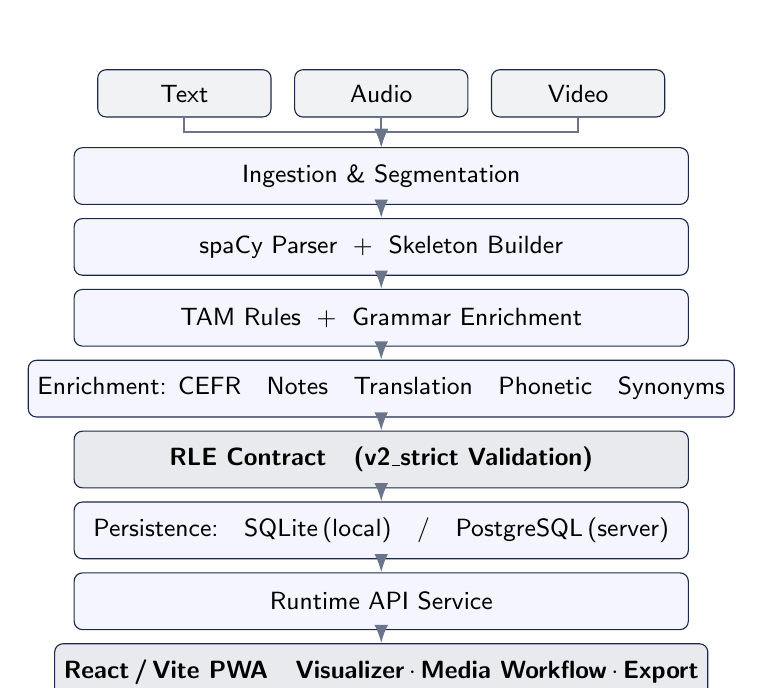
\begin{tikzpicture}[
  box/.style={draw=mtunavy, rounded corners=3pt, fill=blue!4,
              minimum width=7.8cm, minimum height=0.72cm, text centered,
              font=\small\sffamily},
  headerbox/.style={draw=mtunavy, rounded corners=3pt, fill=mtunavy!10,
              minimum width=7.8cm, minimum height=0.72cm, text centered,
              font=\small\bfseries\sffamily},
  inputbox/.style={draw=mtunavy, rounded corners=3pt, fill=mtunavy!6,
              minimum width=2.2cm, minimum height=0.60cm, text centered,
              font=\small\sffamily},
  arr/.style={->, >=Latex, thick, color=mtunavy!65}
]
\node[inputbox] (ntxt) at (-2.5, 0)  {Text};
\node[inputbox] (naud) at ( 0,   0)  {Audio};
\node[inputbox] (nvid) at ( 2.5, 0)  {Video};

\node[box]       (ningest) at (0,-1.05) {Ingestion \& Segmentation};
\node[box]       (nspacy)  at (0,-1.95) {spaCy Parser \;+\; Skeleton Builder};
\node[box]       (ntam)    at (0,-2.85) {TAM Rules \;+\; Grammar Enrichment};
\node[box]       (nenrich) at (0,-3.75)
  {Enrichment: CEFR\quad Notes\quad Translation\quad Phonetic\quad Synonyms};
\node[headerbox] (nrle)    at (0,-4.65)
  {RLE Contract\quad (v2\_strict Validation)};
\node[box]       (nstor)   at (0,-5.55)
  {Persistence:\quad SQLite\,(local)\quad /\quad PostgreSQL\,(server)};
\node[box]       (napi)    at (0,-6.45) {Runtime API Service};
\node[headerbox] (nfront)  at (0,-7.35)
  {React\,/\,Vite PWA\quad Visualizer\,$\cdot$\,Media Workflow\,$\cdot$\,Export};

\draw[arr] (ntxt.south) -- ++(0,-0.18) -| (ningest.north);
\draw[arr] (naud.south) -- (ningest.north);
\draw[arr] (nvid.south) -- ++(0,-0.18) -| (ningest.north);
\draw[arr] (ningest.south) -- (nspacy.north);
\draw[arr] (nspacy.south)  -- (ntam.north);
\draw[arr] (ntam.south)    -- (nenrich.north);
\draw[arr] (nenrich.south) -- (nrle.north);
\draw[arr] (nrle.south)    -- (nstor.north);
\draw[arr] (nstor.south)   -- (napi.north);
\draw[arr] (napi.south)    -- (nfront.north);
\end{tikzpicture}
\caption{High-level architecture of the implemented ELA system}
\end{figure}

\section{Technology Stack}
\begin{table}[H]
  \centering
  \caption{Representative technology stack of the current ELA implementation}
  \begin{tabularx}{\textwidth}{>{\bfseries}p{3.6cm}X X}
    \toprule
    Layer & Main technologies & Role in the system \\
    \midrule
    Frontend & React, Vite, TypeScript, PWA packaging & learner-facing workflow, visualizer, file/project interaction \\
    Desktop packaging path & Tauri & desktop-oriented delivery path alongside the web application \\
    Runtime/API & Python runtime service, HTTP bridge & sentence-contract processing, media submission, job orchestration \\
    Linguistic core & spaCy, deterministic skeleton builder, TAM rules & structural truth layer \\
    Generated enrichment & controlled note-generation path, template transformation, optional T5-based rendering & user-facing pedagogical wording \\
    Translation and speech & M2M100, Whisper, espeak-ng, ffmpeg-related media tools & translation, ASR, phonetics, subtitle/media processing \\
    Storage & SQLite and PostgreSQL paths & local state, persisted analysis history, reproducibility \\
    Deployment & Docker Compose, Nginx & service isolation and reproducible deployment boundaries \\
    \bottomrule
  \end{tabularx}
\end{table}

\section{Backend Linguistic Pipeline}
The core pipeline is implemented in Python under the \texttt{ela\_pipeline} package. The project README and module structure indicate a rules-first design with the following major stages:
\begin{enumerate}
  \item input ingestion and segmentation;
  \item parser-backed skeleton construction;
  \item deterministic TAM enrichment;
  \item optional CEFR, note, translation, phonetic, and synonym enrichment;
  \item contract validation;
  \item persistence and export.
\end{enumerate}

One of the most important architectural decisions is that structural truth is not delegated to a generative model. Parser output, rule logic, and validators form the trust boundary, while generated content is treated as controlled enrichment.

\begin{table}[H]
  \centering
  \caption{Rules-first ownership in the implemented ELA pipeline}
  \begin{tabularx}{\textwidth}{>{\bfseries}p{3.7cm}X X}
    \toprule
    Layer & Main responsibility & Why this matters \\
    \midrule
    spaCy + skeleton builder & structural graph, sentence/phrase/word hierarchy, POS, dependency-backed spans & keeps core representation deterministic and inspectable \\
    TAM rules & tense, aspect, mood, voice, finiteness, TAM construction logic & prevents free-form generation from inventing grammar labels \\
    Tabular or classifier path & CEFR-oriented predictive enrichment and blueprint support & separates classification from free-form wording \\
    Controlled renderer / note path & lexical realization of learner-facing note text & constrains generation to wording rather than structure \\
    Validator & contract safety, schema enforcement, field ownership boundaries & enforces architectural discipline across all later stages \\
    \bottomrule
  \end{tabularx}
\end{table}

\section{Runtime Service and API Layer}
Beyond offline inference scripts, the current system includes a dedicated runtime layer responsible for project management, client storage, media submission, background processing, UI state, and an HTTP bridge for the frontend. This is a significant step beyond the earlier thesis, which focused more on conceptual architecture than on operational service boundaries.

The runtime layer also reveals one of the current weaknesses of the project: the service has become strict enough to expose inconsistencies between expected frontend payloads and actual sentence-node shapes. That makes the runtime layer useful both as an application service and as a form of architectural pressure test.

The runtime API is concrete enough to describe as a product boundary rather than an internal helper. The deployment documentation lists endpoints for project creation, selected-project state, file registration, media submission, backend-job status, visualizer payload retrieval, and edit application. This matters for the thesis because it shows that the implementation phase did not stop at ``produce JSON'' --- it built a service layer through which the learner workflow could actually operate.

\begin{table}[H]
  \centering
  \caption{Representative runtime/API responsibilities described in the current project documentation}
  \begin{tabularx}{\textwidth}{>{\bfseries}p{4.1cm}X}
    \toprule
    Runtime concern & Role \\
    \midrule
    Project and file state & manage learner projects, selected project state, and media registration \\
    Sentence-contract path & expose text-to-contract processing through HTTP endpoints \\
    Media submission & route uploads through local processing or policy-based rejection paths \\
    Background job handling & support long-running tasks and status polling for media workflows \\
    Visualizer payload delivery & provide contract trees back to the frontend in UI-facing form \\
    Edit and synchronization layer & preserve local edits, retry paths, and resume-oriented workflow state \\
    \bottomrule
  \end{tabularx}
\end{table}

\section{Frontend}
The frontend is implemented as a React/Vite progressive web application. It organizes the user experience around projects, files, analysis, vocabulary, configuration, and a linguistic visualizer. Compared with the earlier Kivy-centred prototype framing, this frontend reflects a move toward a more modern web-oriented delivery model and a clearer separation between presentation and processing.

The frontend development note is particularly useful because it records the practical scope of what was actually implemented. It confirms a project-first flow of `Projects -> Files -> Analyze', project-scoped file registration, stage progress reporting, artifact download actions, sentence-by-sentence visualizer navigation, translation-provider handling, quick node edit controls, and vocabulary export. It also records an important architectural subtraction: backend media-job UI controls were removed after the client-first runtime decision. That kind of removal is as important as any added feature because it shows that the final architecture was shaped by narrowing responsibilities, not only by accumulating them.

\section{PWA and End-to-End Workflow Evidence}
The repository also contains a dedicated PWA integration-test guide intended for pre-deployment verification. That document is useful because it describes the system not as isolated modules but as an end-to-end learner workflow:
\begin{enumerate}
  \item open the application;
  \item register service-worker readiness;
  \item create a project;
  \item upload a real media file;
  \item open the analysis screen;
  \item run the full pipeline from transcription through rendering;
  \item verify the appearance of generated downloadable artifacts.
\end{enumerate}

This is important evidence for the thesis because it shows that the project explicitly tests real browser behaviour and long-running media paths, not only narrow unit-level logic. The same test guide also captures several resolved operational problems, such as model-installation readiness, Vite proxy configuration, service-worker cache staleness, and the move away from FFmpeg drawtext rendering toward a Canvas-based video rendering path. It therefore functions as both a verification checklist and a compact record of implementation lessons learned under real end-to-end conditions.

\section{Media Processing}
The media path extends ELA beyond text. Audio and video flow through extraction, transcription, sentence preparation, optional translation, and artifact rendering. The runtime also includes subtitle generation and media export paths, making ELA a multimodal learning system rather than a text-only analysis tool.

The implementation record shows that this path changed materially during development. Earlier stages experimented with backend-oriented media jobs, but the client-first product specification and later implementation artifacts narrowed the architecture toward local processing for interactive media work, explicit duration and file-size gates, and clearer offline and online behaviour. This is a significant architectural result because it demonstrates that multimodality was not simply bolted on; it forced the project to make explicit decisions about privacy, runtime capability, failure boundaries, and where heavy processing should live.

\section{Persistence and Export}
The project contains both local client-side persistence and backend-oriented repository layers, with SQLite and PostgreSQL paths represented in the codebase. Export formats include JSON, CSV, and subtitle artifacts. This persistence strategy supports reproducibility, resumability, and inspection outside the application.

The persistence story is also historically meaningful. Implementation artifacts and product notes show a move from lightweight local repositories toward a more explicit split between device-local workspace state and backend-backed shared or synchronized state. That split helps explain several later design choices: selected-project persistence in the frontend, local edit capture, resumable media workflows, and the minimal-identity policy documented for backend deployment.

\section{Contract Safety as an Architectural Principle}
The technical specification dated 2026-03-20 is explicit that the next-stage architecture should remain classifier-first and contract-safe. In that design, the linguistic contract is not free-form model output but the source context from which later rendering is derived. This leads to clear ownership boundaries: the generator may realize wording, but it must not overwrite structural fields such as node identifiers, parent links, source spans, dependency fields, grammar classes, or CEFR predictions. That separation is one of the strongest engineering ideas in the project because it ties explainability to field ownership rather than to UI rhetoric alone.

\section{Deployment and Service Boundaries}
The Docker deployment documentation shows that ELA is no longer just a local research script collection. The intended deployed form has three clear service boundaries:
\begin{itemize}
  \item PostgreSQL for persistent storage;
  \item an application container for inference, runtime APIs, and migrations;
  \item a frontend container serving the React interface through Nginx.
\end{itemize}

The same documentation also avoids overclaiming. It explicitly distinguishes \texttt{online} and \texttt{offline} runtime modes, notes that model downloads may be disabled at runtime, and states that some features are unavailable in stricter offline or distributed policies. It also makes deployment policy visible as part of the architecture itself through environment-level constraints for media duration, media size, phonetic availability, deployment mode, and runtime download permissions. This is exactly the kind of nuance the final thesis should keep, because it turns ``offline-first'' and ``privacy-first'' from slogans into constrained operational modes with explicit trade-offs.

\chapter{Dataset and Corpus Engineering}
\section{Why Dataset Engineering Matters}
The implemented system is not driven by a single end-to-end model. As a result, dataset engineering plays a different role across subsystems. CEFR estimation, note generation, and future model directions each depend on curated and interpretable training material rather than on generic scraped corpora alone.

\section{Source Families}
The repository indicates several source families and dataset-building paths, including curated corpora, open linguistic resources, and derived educational examples. The codebase and documentation reference sources such as UD-style corpora, OANC, Gutenberg-derived material, MASC, and rulebook or handbook extraction pipelines.

The cumulative book-processing summaries show that this source work was substantial rather than illustrative. In the source-first cumulative summary version v5, the repository records 11 processed book families, 16,248 raw pairs, 14,740 clean pairs, and 8,412 final rows after later row selection, with strong variation by source. For example, the summary attributes 2,746 rows to the Oxford Dictionary path, 2,222 to the Cambridge Dictionary path, and 1,835 to English Grammar Today. These counts matter because they show that the dataset story is not limited to one textbook or one synthetic source; it is the result of repeated extraction and cleaning passes over multiple pedagogical resources.

\section{Curation and Stabilization}
The curator progress report presents the project as having reached a more stable baseline through five linked improvements:
\begin{enumerate}
  \item formalization of a v2-compatible contract;
  \item cleaner phrase structure and stronger fallback-note behaviour;
  \item stricter validation modes and more reliable schema enforcement;
  \item expanded test coverage;
  \item synchronization of documentation with implemented behaviour.
\end{enumerate}

Whether one accepts the phrase ``production-ready baseline'' in full or not, the report captures the intended direction of the implementation phase: less noise, more traceability, and stronger safety around the contract itself.

\section{Deduplication and Quality Control}
A recurring theme in the project documentation is that raw volume is not enough. The system places substantial effort into:
\begin{itemize}
  \item filtering and capping repeated targets;
  \item excluding low-quality or telemetry-like note text;
  \item preserving CEFR balance and grammar-class coverage;
  \item validating note suitability and trace fields;
  \item reducing datasets to examples that remain useful after strict normalization.
\end{itemize}

The practical effect of this policy is visible in the processed dataset statistics. One hybrid T5 contract-target dataset built from the projected corpus started with 2,510 rows and ended with only 380 rows after deduplication and balancing, with 2,130 rows skipped by target-cap controls alone. This is a clear sign that the project prioritized controllable target diversity over raw size. It also explains why some intermediate model results remained weak: the engineering decision to compress and normalize the target space trades scale for discipline.

\section{Placeholder Construction}
The note-generation path depends critically on converting enriched linguistic structures into more abstract templates. This is the point where dataset engineering and the context--pattern duality meet: the abstraction strategy is not only a training trick but part of how the project reframes the pedagogical signal.

The canonical process document dated 2026-03-21 makes that transformation explicit. It defines a ten-step path from book-derived \texttt{notation + content} pairs to inference-time rendering:
\begin{enumerate}
  \item extract notation and paired content from source material;
  \item build a contract tree from the content;
  \item analyze the notation and convert it into placeholder-based template text;
  \item constrain placeholders to attributes available in the paired contract;
  \item train on templated notation rather than on fully rendered final notes;
  \item at inference time, rebuild the contract for new content;
  \item let the model output a notation template with allowed placeholders only;
  \item fill those placeholders from the contract;
  \item write the rendered note back into the tree.
\end{enumerate}

This is a stronger and more specific claim than ``the system uses placeholders.'' It shows that placeholders are intended to sit at the centre of the full data path from source extraction to runtime note realization.

The later slot-normalized projection artifacts make this even more concrete. In the v17 slot-normalized projection report, the repository records 3,505 projected rows, including 1,984 sentence-level slot-templated rows and 6,584 phrase-level slot-templated rows, with additional lexicalized-note repairs recorded explicitly. This demonstrates that placeholder construction was not only a conceptual strategy; it was operationalized as a measurable transformation stage over a large projected corpus.

\section{Template Opportunity Analysis}
The repository also contains reports that measure not just what was extracted but what remained uncovered by the current template inventory. A template-opportunities report over the slot-normalized projection records 513 exact sentence families in projection, of which 205 had book notes and 202 already had book slot templates. The same report identifies phrase families with much weaker template coverage, especially around relative-clause-heavy phrase patterns. This matters because it shows that dataset engineering in ELA included gap analysis, not only corpus growth. The project did not simply build a dataset and train on it; it also measured where the current template space failed to cover the observed grammar families.

\section{Measured Template Space}
The classification-oriented template datasets show that even the template inventory itself was treated as a measurable object. One sentence-multilabel template dataset built from the covered projection reports 1,774 rows after filtering, 48 total template identifiers, 42 sentence template types, and 6 phrase template types. These counts matter because they convert the abstract idea of ``template diversity'' into something inspectable. They also help explain why some model and coverage decisions in later chapters could be made with more confidence: the project had begun to quantify the shape of its pedagogical pattern space rather than relying on intuition alone.

\section{From Free-Form T5 to Controlled Rendering}
The project documentation shows a clear evolution away from unconstrained note generation. By March 2026, the preferred architecture was no longer ``raw text to T5 note.'' The intended flow had become:
\begin{enumerate}
  \item validated linguistic contract;
  \item deterministic structural enrichment;
  \item CEFR prediction and blueprint generation;
  \item contract-to-template transformation;
  \item controlled lexical realization from that template;
  \item post-render validation confirming that classifier-owned and contract-owned fields remain unchanged.
\end{enumerate}

This evolution is important for the thesis because it supports a more mature claim than ``the system uses T5.'' The stronger claim is that generation is being progressively confined to the narrowest part of the problem where wording variation is desirable but structural drift is unacceptable.


\section{How the Dataset Strategy Evolved: From Raw Corpora to Grammar Books}
\label{sec:closed-pipeline}
The dataset construction strategy reached its current form through several distinct phases, each motivated by a concrete limitation discovered in the previous one. Understanding this evolution is important because the final ``closed'' architecture is not an initial design choice but the result of iterative problem-solving.

\subsection*{Phase 1: Raw Corpora and Free-Form Generation}
The earliest dataset version ingested open-licence corpora---UD English Web Treebank, OANC, Tatoeba, and Wikinews---producing around 3,000 sentences and their parsed representations. T5 was trained to output a free-form pedagogical note given a spaCy contract describing the sentence. Notes were unconstrained: the model could write anything. The variability of output appeared high, but inspection revealed that the model quickly converged on a small set of generic phrasings that were technically grammatical but offered little pedagogical value.

\subsection*{Phase 2: Grammar Blueprints}
To stabilize output quality, the project introduced a library of over 150 \emph{grammar blueprints}---hand-written, rule-based note templates keyed to specific grammatical classes such as \texttt{present\_simple\_affirmative}, \texttt{relative\_clause}, or \texttt{passive\_voice}. Each blueprint provided a fixed note at three CEFR tiers (elementary, intermediate, advanced). Blueprints served as a deterministic fallback when model output failed quality gates. The approach improved consistency, but the inverse problem became clear: the blueprint library itself was too coarse. The same note appeared thousands of times in the projected corpus, and the model had no incentive to learn anything except which blueprint to select.

\subsection*{Phase 3: Slot-Based Templates}
The next step was to parametrize blueprints with named placeholders. Instead of a fixed string, a note template could contain \texttt{\{\{HEAD\_NOUN\}\}}, \texttt{\{\{PREPOSITION\}\}}, \texttt{\{\{OBJECT\_NP\}\}}, or \texttt{\{\{RELATIVE\_MARKER\}\}}---fields resolved at projection time from the linguistic contract of the matched instance. This made each template potentially produce a distinct note for every sentence it matched. The technical infrastructure for this---slot validation, contract-to-slot resolution, template registry---was introduced in March 2026 and is described in more detail in the Placeholder Construction section above. The placeholder system worked, but exposed a new bottleneck: the repository contained only a few dozen manually authored template variants. Corpus projection amplified those templates across many sentences, but the underlying pattern space remained narrow.

\subsection*{Phase 4: Grammar Books as the Source of Patterns}
The diagnostic finding, documented explicitly in the template expansion strategy report for v16, was that \emph{the main bottleneck is insufficient template granularity}. The solution was to stop authoring templates manually and instead extract them from existing pedagogical sources. Specialized grammar handbooks---Collins COBUILD English Grammar, George Yule's \emph{Explaining English Grammar}, Betty Azar's \emph{Basic English Grammar}, Mark Lester's \emph{English Grammar Drills}, Farlex \emph{Complete English Grammar Rules}, and others---contain thousands of author-written explanations, each paired with a curated example sentence. These are exactly the slot templates the project needed: validated by domain experts, covering a wide range of constructions, and already matched to example sentences that could drive the contract extraction step. A book extraction engine was built to parse EPUB, PDF, and DJVU formats and output the same notation--content pair format used throughout the pipeline.

\subsection*{Canonical Training and Inference Flow}
The canonical process for book-to-dataset-to-inference, documented explicitly on 2026-03-21, fixes the full flow in ten steps. The first six steps produce the training dataset; the last four describe what happens at inference time for a new sentence.

\textit{Training path (steps 1--6).} A grammar book provides pairs of \emph{notation} (the author's pedagogical explanation) and \emph{content} (the example sentence). The content is parsed by spaCy into a linguistic contract tree. The notation is analysed and converted into a \emph{template}: the same explanation text, but with content-specific terms replaced by named placeholders such as \texttt{\{\{HEAD\_NOUN\}\}} or \texttt{\{\{PREPOSITION\}\}}. Placeholders may reference only attributes that exist in the contract built from the paired content---the contract is the sole source of allowed slot values. Each book pair then becomes one T5 training row: the input is the contract context together with the template structure; the \emph{target is the template text with placeholders intact}, not the rendered final note.

\textit{Inference path (steps 7--10).} When a new sentence arrives from a user, it passes through the same spaCy parser, producing a contract with the same schema as the training contracts. The T5 model, trained on templated targets, outputs a notation template with placeholders. Those placeholders are then filled from the very same contract that was the model's input---the contract serves double duty as both the generation context and the slot-value source. The filled template is the rendered pedagogical note, saved back into the contract tree under \texttt{linguistic\_notes}.

This symmetry---the contract is the context at training time, and the same contract schema provides the slot values at inference time---is the technical foundation of controlled note generation. The model never sees raw unbounded text as a target and never invents structure; it only realises wording for a template derived from and constrained by the contract.

\subsection*{Field Ownership}
The architecture formalises ownership of every contract field across three layers, as fixed in the field ownership document dated 2026-03-04:

\begin{itemize}
  \item \textbf{spaCy and deterministic rules} own all structural fields: the tree shape, node types, part of speech, dependency labels, morphology, TAM fields (tense, aspect, mood, voice, finiteness), grammar classes, and note blueprints. These fields are set once and cannot be modified by any downstream model.
  \item \textbf{Tabular ML (XGBoost)} owns \texttt{cefr\_level}. This is the only field produced by a trained classifier in the production path. It is treated as a prediction, not as structural truth, and is never overwritten by the note generation step.
  \item \textbf{T5} owns only \texttt{linguistic\_notes}---the user-facing wording. It receives the blueprint text (derived from grammar classes) and the contract context as input; it may only produce note text. It is explicitly forbidden from changing any classifier-owned or structure-owned field.
\end{itemize}

This ownership matrix is the reason the system is called \emph{contract-safe}: the contract is not a free-form generation output but a structured record whose fields are owned by specific, accountable sources.

\subsection*{Three-Tier CEFR Note Design}
A deliberate three-tier design governs how note templates are treated at different proficiency levels:

\begin{itemize}
  \item \textbf{Elementary (A1--A2)}: fixed passthrough templates. Notes describe simple, unambiguous rules that do not vary with the surface content of the matched sentence. They serve as a lower-bound baseline in evaluation.
  \item \textbf{Intermediate (B1--B2)}: slot-templated generation. This is the primary generation task, where the same abstract pattern produces a different, grounded note for each matched sentence via contract-driven slot filling.
  \item \textbf{Advanced (C1--C2)}: fixed passthrough templates. Notes describe complex, construction-level rules that are likewise invariant to surface content, acting as an upper-bound comparison baseline.
\end{itemize}

By treating the boundary tiers as fixed, the project creates two natural comparison groups that bracket the range achievable by the generation system. Concrete examples from the actual training data are provided in Appendix~\ref{app:pipeline-examples}.

\chapter{Evaluation}
\section{Evaluation Approach}
The evaluation of ELA must be understood as layered rather than singular. No single metric validates the entire system. Instead, different subsystems require different forms of evidence:
\begin{itemize}
  \item contract validity and structural correctness;
  \item CEFR prediction quality;
  \item pedagogical note generation quality;
  \item media pipeline behaviour;
  \item end-to-end runtime usability.
\end{itemize}

\section{Evaluation Method}
The thesis uses a mixed evidence strategy rather than a single benchmark suite. Evaluation evidence is drawn from:
\begin{itemize}
  \item structured project documents describing architectural intent and pipeline evolution;
  \item sample contract artifacts and schema definitions;
  \item explicit evaluation JSON and report checkpoints;
  \item broad unit-test coverage across classifier, runtime, media, contract, and validation layers;
  \item targeted reproduction of failing tests in the current codebase to identify active regressions.
\end{itemize}

This approach is appropriate for the current state of ELA because the project is simultaneously a research artifact, a software system, and a still-evolving product. A thesis that ignored any one of those layers would misrepresent the actual nature of the work.

\section{What the Current Evidence Supports}
The project contains substantial test infrastructure and multiple evaluation artifacts. This supports several defensible conclusions:
\begin{itemize}
  \item the codebase is not a loose prototype but a systematically exercised system;
  \item CEFR and note-generation paths were treated as measurable modelling problems rather than hand-waved add-ons;
  \item media, runtime, and persistence layers were tested as first-class concerns.
\end{itemize}

\section{Classifier Path and Controlled Generation Evidence}
One useful checkpoint in the repository is the phase-1 classifier execution report dated 2026-02-25. That report confirms an orchestrated training and quality-cycle run, classifier metadata generation, runtime sentence-contract validation, and controlled note rewriting behaviour. At the same time, the report also reveals a limitation that is academically important: the baseline freeze at that point still used a very small training set. This means the existence of the pipeline is strongly supported, while any broad performance claim should remain tied to the exact dataset version that produced it.

This early checkpoint becomes much more informative when read together with later classifier artifacts. The repository contains a progression from this tiny baseline freeze toward a substantially larger full-ladder tabular run. That progression matters because it shows that the classifier path did not remain a proof of concept; it was scaled, compared, and stress-tested as the project matured.

\section{Concrete Tabular Evaluation Snapshot}
Another useful artifact is the full-ladder tabular evaluation snapshot dated 2026-03-05. Unlike broad narrative claims, this file gives a concrete checkpoint with explicit split sizes and summary metrics:

\begin{table}[H]
  \centering
  \caption{Selected values from the 2026-03-05 tabular joint-profile evaluation artifact}
  \begin{tabular}{lr}
    \toprule
    Metric or count & Value \\
    \midrule
    Training rows & 8211 \\
    Development rows & 1182 \\
    Test rows & 1196 \\
    Joint development accuracy & 0.9797 \\
    Joint test accuracy & 0.9849 \\
    Grammar development macro-F1 & 0.8088 \\
    Grammar test macro-F1 & 0.8231 \\
    Runtime smoke check & pass \\
    \bottomrule
  \end{tabular}
\end{table}

This snapshot is useful for two reasons. First, it proves that at least one later evaluation stage moved far beyond the tiny baseline freeze described in the February phase-1 report. Second, it shows why metric claims must be attributed carefully: different documents in the repository reflect different phases, datasets, and evaluation scopes. For the thesis, the safest strategy is to treat metrics as checkpoint-specific rather than as timeless project constants.

\section{Comparative Evidence and Intermediate Results}
The evaluation story becomes stronger when intermediate and comparative artifacts are treated as part of the evidence rather than dismissed as noise. For example, the March 2026 comparison between the tabular full-ladder path and the DeBERTa-based full-ladder path shows that the tabular route became the stronger practical choice for the production-oriented stack. In that comparison, the DeBERTa CEFR-only hygiene smoke result achieved only 0.1612 accuracy and 0.0463 macro-F1, collapsing almost all predictions to the `C1` class. This is a valuable engineering result because it explains why the project moved away from treating the heavier classifier path as the obvious runtime default.

The note-generation artifacts tell a similarly important story. Intermediate T5 evaluation reports in directories such as \texttt{results\_llm\_notes\_refresh\_data\_processed\_e2} show structurally valid training and evaluation runs, but still very weak exact-match behaviour on the measured target space. Earlier template-id and refresh experiments therefore matter as negative evidence: they show that simply running T5 over a notation-like target did not automatically produce useful pedagogical output. The later placeholder and controlled-rendering direction should be understood as a response to those weak intermediate results rather than as an arbitrary conceptual preference.

This layered reading of the artifacts is important for the thesis. A convincing evaluation chapter should not present only the best surviving checkpoint. It should show that the project made decisions in response to evidence: weak template-id target diversity, weak practical fallback behaviour, tiny early classifier datasets, failed or underperforming comparative routes, and then stronger later checkpoints that justified a narrower architecture.

\section{What the Current Evidence Does Not Fully Support}
At the same time, the current development state also places important limits on the thesis claims. The current codebase is not fully green under the project's own unit-test suite. Targeted failures remain in:
\begin{itemize}
  \item node-level translation propagation;
  \item phrase and sentence skeleton behaviour;
  \item validation-mode consistency around TAM fields;
  \item ASR sentence resegmentation and metadata filtering;
  \item parts of the runtime-service integration boundary.
\end{itemize}

This matters because it affects how evaluation should be written. The system can be defended as substantial and technically serious, but not as fully stabilized across every path.

\section{Representative Findings from Review}
The implementation review identified the following representative engineering realities:
\begin{itemize}
  \item the runtime layer strongly validates frontend-visible payloads, which is architecturally good, but currently exposes payload-shape mismatches;
  \item the skeleton builder remains a critical subsystem, and regressions there have direct pedagogical consequences because phrase structure is learner-visible;
  \item translation quality is not only a linguistic issue but also a structural one, because wrong projection to child nodes changes what the learner sees as local meaning;
  \item the media path is operationally ambitious, but multimodal support is more fragile than the text path.
\end{itemize}

\section{Overall Assessment}
Overall, the project evaluates well as a research-engineering system:
\begin{itemize}
  \item it is broad enough to demonstrate full-stack integration;
  \item it is deep enough to support concrete architectural and modelling discussion;
  \item it is honest enough, when reviewed carefully, to show the gap between implemented ambition and production hardening;
  \item it preserves enough intermediate evidence to explain why later design decisions were made.
\end{itemize}

\section{End-to-End Integration Perspective}
The PWA integration documentation provides one more useful perspective on evaluation. It identifies concrete failure classes that unit tests alone may miss: browser-side model availability, service-worker cache drift, ffmpeg-related rendering failures, missing proxy headers, and user-flow stalls during long-running media processing. For the thesis, this broadens the meaning of ``system validation.'' In ELA, validation is not only about linguistic correctness; it is also about whether a learner can move from upload to usable artifact through a stable interface path.

\section{Objectives-to-Evidence View}
\begin{table}[H]
  \centering
  \caption{High-level objective-to-evidence mapping for the current thesis}
  \begin{tabularx}{\textwidth}{>{\bfseries}p{2cm}X X}
    \toprule
    Objective & Intended outcome & Current evidence type \\
    \midrule
    O1 & Multimodal pipeline from text/audio/video to sentence-level analysis & runtime modules, integration-test guide, API/service code, unit tests \\
    O2 & Stable hierarchical contract carrying structural and pedagogical metadata & sample contract, validator, schemas, curator report, contract-safe architecture docs \\
    O3 & Learner-facing interface for exploration, export, and workflow control & React/Vite frontend, runtime API endpoints, visualizer-related implementation artifacts and docs \\
    O4 & Improved note-generation generalization through structural abstraction & template-process docs, template-expansion strategy, T5/placeholder narrative in project docs \\
    \bottomrule
  \end{tabularx}
\end{table}

\chapter{Discussion, Limitations, and Future Work}
\section{Discussion}
The implemented ELA system supports the central thesis direction: authentic language can be made more accessible through layered structural explanation rather than through simplification. The combination of hierarchical representation, deterministic truth layers, and learner-facing visualization remains the strongest and most coherent aspect of the project.

The most interesting deeper result is that abstraction appears to matter more than raw model complexity in pedagogical generation. The placeholder-based route suggests that the project achieved its clearest modelling gains not by escalating model size but by refining representational form. In practical terms, the project moved from asking a model to memorize many surface realizations toward asking it to learn a more stable mapping between structural context and explanatory pattern.

This is also where the engineering and research layers of the thesis meet most clearly. The same design instinct that pushed the runtime toward stricter contracts and deterministic boundaries also pushed the note-generation path toward canonicalized training signals. In both cases, the project became stronger when implicit variation was converted into explicit structure.

\section{From LLM Pattern Learning to a General Scientific Method:
         A Pattern-Sequence Hypothesis}

The hypothesis formalised in this section did not originate as an abstract theoretical claim.
It emerged through a sequence of practical observations during the ELA implementation work
and was subsequently confirmed in a second, physically unrelated domain.
The fact that the same core idea surfaced independently in two domains---natural language
pedagogy and meteorological forecasting---is what elevates it from an engineering note to
a candidate general principle.

\subsection*{Origin in the ELA Pipeline Failure}

The first encounter with the principle came from a practical failure rather than a design
intention. When the training signal for the T5 note-generation path preserved full lexical
surface detail, the model overfit to specific examples rather than learning transferable
pedagogical patterns. The template-ID experiment of February 2026 made this concrete: after
target-space balancing, the effective target inventory collapsed to only ten unique template
identifiers, and the fallback rate on the small regression probe reached 1.0. The model had
learned nothing useful because the surface form carried more variation than the structure---
and the model, given no incentive to the contrary, memorised the variation rather than
the underlying pattern. The corrective move---replacing raw notation with
placeholder-bearing structural templates---produced qualitatively different behaviour.
The model began to generalize across vocabulary while preserving grammatical interpretation.
This was the first empirical encounter with the claim: the structural pattern, not the
surface form, carries the transferable signal.

\subsection*{A Historical Precedent: Mendeleev's Grammar}

The intellectual analogy that clarifies this observation most sharply predates machine
learning by more than a century. Mendeleev did not discover new chemical elements. What he
discovered was that elements, when arranged by their intrinsic properties,
\emph{form repeating patterns}---and that those patterns are predictive. When the
sequence of known elements violated the expected structure, he did not discard the anomaly.
He left an empty cell and predicted the properties of the missing element from the
constraints imposed by its position in the pattern. The element was subsequently found.

The method, stripped of its chemical content, consists of three steps: identify the minimal
analytical unit of description appropriate to the domain, classify it, study the grammar
of its sequential arrangements, and use that grammar to forecast. The Periodic Table is not
a list of elements; it is a grammar of elemental transitions. This is precisely what the
ELA and weather forecasting projects each implement in their respective domains. In neither
case does the model learn to predict the raw surface. In both cases, it learns to predict
the \emph{type and structure of the next analytical unit} in a sequential grammar.

\subsection*{Language as the First Domain}

In ELA, the analytical unit is the Recursive Linguistic Element node. Each sentence, phrase,
and word node is described not by its specific lexical content but by its structural type,
grammatical role, tense-aspect-mood classification, and position in the hierarchy. The
placeholder-based training signal then asks the model to predict which structural pattern
applies to a new example---which note template, which grammatical regime---rather than
to memorise which words appeared in training. This is the open phase of the duality: many
contextual examples, each with different surface vocabulary, carve a stable internal pattern
space. In the closed inference phase, the frozen pattern then imposes structure on whatever
new context arrives. This statement is formulated explicitly in the core hypothesis:

\begin{quote}
Effective training of an LLM is achieved when both the input and the output are represented
as patterns with placeholders, and variability is realised not as a separate collection of
individual cases, but as a structured system of filling those placeholders within the
pattern.

This gives rise to the hypothesis that, in open systems, context forms patterns, whereas in
closed systems, stable patterns structure the permissible context of their realisation.

In turn, this suggests that the complexity of natural systems is determined not by an
infinite multitude of variants, but by a limited set of stable patterns through which those
variants become possible, reproducible, and interpretable.
\end{quote}

\subsection*{Weather Forecasting as the Second Domain}

The most direct external evidence for the generality of this approach comes from parallel
work on single-station meteorological forecasting~[15] conducted at Knock Airport, Ireland,
using Met \'{E}ireann historical hourly data covering the period 2020--2026. In that system, raw
sensor measurements are not fed directly to a model. Instead, the time series is first
segmented into analytical intervals, each described by one of a small library of
ODE-derived equation types: \texttt{constant}, \texttt{linear}, \texttt{exponential},
\texttt{harmonic}, and \texttt{damped\_harmonic} for temperature, and a three-type
vocabulary for pressure and wind speed. The choice of equation type and its fitted
parameters constitute the vocabulary of meteorological regimes in precisely the same sense
that RLE node types constitute the vocabulary of grammatical regimes in ELA.

A transformer encoder is then trained to predict the \emph{sequence} of future ODE segment
descriptors from a window of past ones. The model receives no atmospheric physics, no
spatial observations, and no numerical weather prediction output. It learns only the
sequential grammar of analytical meteorological units from six years of a single station's
history. On a seven-day evaluation period in February 2026, the ensemble achieves a
pressure mean absolute error of 0.89~hPa at the 12-hour horizon, a 34\% improvement
over naive persistence (1.35~hPa), using no domain physics whatsoever. This is not a
claim of superiority over operational numerical weather prediction systems; it is a proof
of concept that the \emph{grammar of physical regimes is learnable from sequential
analytical units alone}, exactly as the grammar of linguistic regimes proved learnable in
ELA.

The structural parallel between the two domains is summarised in Table~\ref{tab:domainparallel}.

\begin{table}[H]
  \centering
  \caption{Structural parallel between the ELA and weather forecasting pattern-sequence approaches}
  \label{tab:domainparallel}
  \begin{tabularx}{\textwidth}{>{\bfseries}p{3.5cm}X X}
    \toprule
    Concept & ELA (language domain) & Weather forecasting domain \\
    \midrule
    Analytical unit &
      RLE node (sentence, phrase, word) &
      ODE segment (constant, linear, exponential, harmonic) \\
    Unit descriptor &
      type, TAM, grammatical role, CEFR level &
      equation type, fitted parameters, duration \\
    Sequence model &
      transformer over RLE node sequences &
      transformer over ODE segment sequences \\
    Training signal &
      structural templates with placeholders &
      segment descriptor vectors \\
    Predicted output &
      next structural pattern and its template slots &
      next segment type and fitted parameters \\
    Decoded output &
      learner-facing pedagogical note &
      hourly meteorological forecast values \\
    \bottomrule
  \end{tabularx}
\end{table}

\subsection*{Formulation of the General Method}

These two cases suggest a three-step method that may apply to any sufficiently regular
natural or artificial process:

\begin{enumerate}
  \item \textbf{Decompose.}
        Identify the minimal analytical unit of description appropriate to the domain.
        The unit should be expressive enough to capture the essential structure of a
        regime, compact enough to form a finite vocabulary, and grounded in domain
        knowledge rather than derived purely from statistical clustering.
        In language, the unit is the grammatical node with its TAM and role attributes.
        In meteorology, it is the ODE segment type with its fitted parameters.

  \item \textbf{Classify and sequence.}
        Observe that naturally occurring instances of the process form sequences of these
        units. Classify the units, record their transitions, and treat the sequence as the
        primary object of study rather than the raw surface values.
        The Periodic Table is the canonical example of this step applied to chemistry:
        once elements are classified by their properties, the grammar of their arrangement
        becomes visible and predictive.

  \item \textbf{Learn the grammar and predict.}
        Apply a sequence model to the classified unit stream. Because the model operates
        on analytical descriptors rather than raw measurements, it learns the structural
        regularities---the grammar---of regime transitions. Predictions are then
        decoded back to surface form through the analytical units themselves, preserving
        interpretability at every step.
\end{enumerate}

\subsection*{A New Methodology of Scientific Inquiry}

The pattern-sequence approach is worth situating not only as a machine-learning technique
but as a methodology of scientific inquiry in its own right---one that became practically
realisable only with the arrival of modern sequence models.
Prior to the transformer era, identifying the analytical units of a domain and studying
their sequential grammar was work reserved for domain experts investing years of manual
analysis. The Periodic Table took Mendeleev a lifetime; the grammatical rules of natural
language occupied generations of linguists; the ODE taxonomy of meteorological regimes
exists only as informal folklore among forecasters.
What the AI revolution makes possible is the \emph{automation of the grammar-learning step}:
once a domain can be expressed as a sequence of interpretable analytical units, a
transformer can extract the sequential regularities from historical data at a scale no human
analyst could match.

This positions the three-step method---decompose, classify, learn the grammar---
as a candidate general framework for data-driven scientific understanding, distinct from
both classical hypothesis-driven science and from the black-box statistical learning that
characterises much of modern deep learning. It is interpretable because the units are
analytically defined; it is powerful because the grammar is learned from data; and it is
generalisable because the same architectural pattern---segment, describe, sequence-model---
applies wherever recurring analytical regimes can be identified. The two domains
examined in this thesis, natural language and meteorology, are early instances of what may
prove to be a broader shift in how structured knowledge is extracted from complex systems.

\subsection*{Scope and Limitations of the Hypothesis}

The hypothesis should be understood as an empirical claim derived from two implemented
cases, not as a formal theorem. Several important qualifications apply.

First, the quality of the analytical decomposition is a decisive factor. If the vocabulary
of units is too coarse, important distinctions collapse; if it is too fine, the model faces
a large and sparsely populated unit space that is difficult to learn from. In both ELA and
the weather project, vocabulary size was determined through domain knowledge and iterative
refinement rather than by automated search, and that design investment is not free.

Second, the generalization gains observed in both domains are bounded by evaluation scope.
ELA's placeholder-based note generation was evaluated on a controlled annotation set; the
weather forecasting result covers one week at one station during a challenging frontal
passage. Neither result is sufficient to claim general superiority over all alternative
approaches.

Third, the claim is not that all complexity reduces to patterns in a mystical sense. The
hypothesis is more practical: in domains where analytical decomposition is feasible, learning
the grammar of analytical unit sequences is a more efficient and more interpretable strategy
than learning directly from raw surface data. Whether that efficiency advantage survives in
richer, noisier, or higher-dimensional domains is an open research question.

The three-step method, the Mendeleev analogy, and the context--pattern duality together
constitute the research contribution of this thesis that extends beyond ELA's engineering
work. They represent a design philosophy tested in two domains and presented here as a
candidate framework for further systematic investigation.

\section{Limitations}
The current limitations are both scientific and engineering-related:
\begin{itemize}
  \item some reported metrics still require careful reconciliation with the precise artifacts that produced them;
  \item the current codebase contains unresolved regressions in the core pipeline;
  \item multimodal support is more fragile than text-only processing;
  \item some claims inherited from earlier project narratives need weaker wording in light of the current implementation state;
  \item the project still lacks a full user-study layer capable of demonstrating educational impact beyond technical plausibility.
\end{itemize}

The repository planning artifacts show that these limits are not abstract caveats added after the fact. Several unfinished items in the working TODO trail correspond directly to the current discussion. Examples include moving \texttt{grammar\_classes} ownership fully into the rules-first runtime path, deciding whether DeBERTa remains a research-only path or is fully retired from the mainline runtime story, and tightening provenance and licensing evidence for some advanced-corpus packages. The remaining work is now relatively concrete: the project is no longer blocked by lack of direction but by stabilization, ownership cleanup, and proof discipline.

\begin{table}[H]
  \centering
  \caption{Current implementation limitations and their practical impact}
  \begin{tabularx}{\textwidth}{>{\bfseries}p{4.1cm}X}
    \toprule
    Limitation area & Practical impact on the thesis or system \\
    \midrule
    Metric fragmentation across phases & prevents careless use of a single headline number for the whole project \\
    Runtime-service payload mismatch & shows that architectural strictness currently outpaces some frontend/runtime integration assumptions \\
    Skeleton and translation regressions & directly affect learner-visible tree quality and node-level interpretation \\
    Multimodal fragility & makes text processing more stable than audio/video processing in the current codebase \\
    Lack of large-scale user study & limits pedagogical claims to technical plausibility and architecture-backed rationale \\
    \bottomrule
  \end{tabularx}
\end{table}

\section{Future Work}
The most immediate future work falls into three clusters:
\begin{enumerate}
  \item \textbf{Stabilization.} Resolve current regressions in skeleton construction, translation projection, runtime validation boundaries, and media sentence preparation.
  \item \textbf{Model path maturation.} Continue the abstraction-based note-generation line, expand dataset evidence, and strengthen the empirical basis of the context--pattern duality claim.
  \item \textbf{Product hardening.} Improve media playback, subtitle synchronization, packaging, deployment consistency, and frontend/runtime ergonomics.
\end{enumerate}

The recent repository evidence suggests that this future work is likely to remain iterative rather than monolithic. Many 2026 implementation passes are not feature additions but corrective passes over translation routing, batch behaviour, provider selection, stale translation cleanup, media caching, and rendering reliability. That pattern implies that the next mature phase of ELA will depend less on adding yet another model and more on reducing boundary mistakes between already existing components.

Beyond those immediate priorities, the documentation also points toward longer-horizon directions: tighter offline packaging of runtime models, richer translation quality gates, broader corpus growth, stronger observability around pipeline failures, more disciplined separation between classification, controlled rendering, and user-facing editing workflows, and eventually a user-study layer that can test whether the explainable interface actually improves learner comprehension and retention under realistic use.

\chapter{Conclusion}
This thesis has presented ELA as the continuation of an earlier research programme into explainable support for authentic English input. The project has evolved from a concept and prototype direction into a substantial full-stack implementation built around the RLE contract, a rules-first linguistic pipeline, multimodal processing, and a learner-facing frontend.

The core technical lesson of the work is twofold. First, explainability requires architecture, not just model output: contracts, validators, runtime boundaries, and structural representations all matter. Second, abstraction in the training signal appears to be a decisive factor in pedagogical note generation, motivating the context--pattern duality as the main interpretive research contribution of this phase, within the limits of the current evidence base.

The project is not finished. Its current codebase still exposes unresolved regressions and integration mismatches, especially in the runtime and multimodal paths. Yet that incompleteness does not weaken the value of the thesis; it clarifies it. ELA is best understood not as a polished consumer product but as a serious research-engineering system whose value lies in what has already been made explicit: a reusable architecture, a contract-centred representation model, a credible multimodal workflow, and a modelling direction that can be tested further rather than merely asserted.

In that sense, the continuation from the earlier research thesis is successful. The original pedagogical vision was not abandoned during implementation; it was forced into concrete interfaces, validators, services, datasets, and failure cases. That transition from concept to accountable system is the real achievement documented in this report.

\appendix

\chapter{Repository Evidence Sources}
Table~\ref{tab:repoevidence} summarises the main repository artifacts used to support the thesis claims. The purpose of this appendix is not to reproduce those documents in full but to make explicit which internal sources informed architectural, evaluative, and historical statements in the main body.

\begin{table}[H]
  \centering
  \caption{Representative repository evidence sources used in this thesis}
  \label{tab:repoevidence}
  \begin{tabularx}{\textwidth}{p{5.2cm}X}
    \toprule
    \textbf{Repository artifact} & \textbf{Thesis role} \\
    \midrule
    Project README set & high-level system narrative, feature inventory, and implementation scope \\
    Full pipeline documentation & broad architectural description of the pipeline and runtime responsibilities \\
    Technical specification dated 2026-03-20 & system-level technical specification and contract-oriented implementation detail \\
    Template expansion strategy v16 & evidence for controlled rendering and placeholder-driven note-generation strategy \\
    Canonical book-to-dataset process note dated 2026-03-21 & evidence for dataset construction and contract-to-template processing flow \\
    Phase-1 classifier execution report dated 2026-02-25 & checkpoint evidence for classifier orchestration and small-baseline limitations \\
    Full-ladder tabular evaluation artifact dated 2026-03-05 & concrete metrics snapshot for later-stage tabular evaluation \\
    PWA integration test note & evidence for end-to-end PWA and runtime interaction testing \\
    Docker deployment note & deployment and packaging evidence for the implementation story \\
    Current unit-test suite and targeted failing tests & evidence for both maturity and unresolved regressions in the present codebase \\
    \bottomrule
  \end{tabularx}
\end{table}

\chapter{Evaluation Artifact Index}
The project contains multiple evaluation checkpoints rather than a single immutable benchmark. Table~\ref{tab:evidencelevels} indexes the main classes of evidence used in the report and clarifies what each can and cannot support in academic terms.

\begin{table}[H]
  \centering
  \caption{Evidence categories and their interpretive strength in the current thesis}
  \label{tab:evidencelevels}
  \begin{tabularx}{\textwidth}{>{\bfseries}p{3.7cm}>{\bfseries}p{3.2cm}X}
    \toprule
    Evidence class & Strength level & Appropriate use in the thesis \\
    \midrule
    Running code and compiled thesis output & High & supports claims that the project exists as an operational software artifact with reproducible document output \\
    Contract schema, validators, and runtime interfaces & High & supports claims about architectural intent, field ownership, and explainability-oriented system design \\
    Evaluation JSON checkpoints and classifier reports & Medium to high & supports checkpoint-specific metric claims when the producing dataset and phase are stated explicitly \\
    Integration tests and runtime smoke paths & Medium & supports claims that cross-layer workflows were implemented and exercised end to end \\
    Targeted failing tests in the current codebase & High for limitations & supports current-state limitation claims and prevents overstating maturity \\
    Earlier thesis and narrative planning documents & Medium & supports continuity and design intent, but not unconditional statements about the current codebase \\
    \bottomrule
  \end{tabularx}
\end{table}


\chapter{Pipeline Template Examples}
\label{app:pipeline-examples}
This appendix provides concrete examples drawn from the actual training data generated by the closed pipeline described in Section~\ref{sec:closed-pipeline}. As explained there, the pipeline uses a three-tier design:

\begin{itemize}
  \item \textbf{Elementary (A1--A2)}: fixed passthrough templates, used as a lower-bound comparison baseline;
  \item \textbf{Intermediate (B1--B2)}: slot-templated generation, the primary modelling target;
  \item \textbf{Advanced (C1--C2)}: fixed passthrough templates, used as an upper-bound comparison baseline.
\end{itemize}

For each example the table shows the source phrase or sentence, the grammatical topic as labelled in the source book, the note template (with any \texttt{\{\{SLOT\}\}} placeholders shown explicitly for intermediate examples), and the final rendered note that would be displayed to the learner.

\subsection*{Elementary Level (A1--A2): Passthrough Notes}

At the elementary tier the note text is typically short, unambiguous, and directly applicable regardless of the specific sentence. These notes are stored as passthrough templates with no slots.

\begin{table}[H]
  \centering
  \caption{Elementary-level passthrough note examples from the training corpus}
  \label{tab:elem-examples}
  \begin{tabularx}{\textwidth}{p{4.2cm}p{3.4cm}X}
    \toprule
    \textbf{Source phrase / sentence} & \textbf{Topic} & \textbf{Note (passthrough template)} \\
    \midrule
    \emph{I'm going to go downtown tomorrow.} & be going to future & Be going to is used to talk about a future plan or intention. \\
    \midrule
    \emph{Ann isn't going to study tonight.} & be going to negative & In negative be going to clauses, not follows be. \\
    \midrule
    \emph{Are you going to come to class tomorrow?} & be going to yes-no question & A yes-no question with be going to is formed by placing be before the subject. \\
    \midrule
    \emph{What time are you going to eat dinner tonight?} & be going to wh-question & A wh-question with be going to begins with the wh-expression and keeps be before the subject. \\
    \midrule
    \emph{There is a book on my desk.} & existential there basic & There is introduces the existence of a singular thing in a place or situation. \\
    \bottomrule
  \end{tabularx}
\end{table}

\subsection*{Intermediate Level (B1--B2): Slot-Templated Notes}

At the intermediate tier many note patterns contain references to specific grammatical elements of the target phrase. These are stored as slot templates; at projection time the slots are filled from the linguistic contract of the matched corpus instance, producing a grounded note for each new context.

\begin{table}[H]
  \centering
  \caption{Intermediate-level slot-templated note examples from the training corpus}
  \label{tab:inter-examples}
  \begin{tabularx}{\textwidth}{p{3.2cm}p{2.6cm}p{3.8cm}X}
    \toprule
    \textbf{Target phrase} & \textbf{Topic} & \textbf{Note template (with slots)} & \textbf{Rendered note (slots filled)} \\
    \midrule
    \emph{that you hit} & relative clause antecedent &
      This relative clause gives more information about the noun ``\{\{HEAD\_NOUN\}\}''. &
      This relative clause gives more information about the noun ``car''. \\
    \midrule
    \emph{that I met} & object relative clause &
      This relative clause gives more information about the noun ``\{\{HEAD\_NOUN\}\}''. &
      This relative clause gives more information about the noun ``woman''. \\
    \midrule
    \emph{that you talked to} & stranded preposition relative clause &
      This relative clause gives more information about the noun ``\{\{HEAD\_NOUN\}\}''. &
      This relative clause gives more information about the noun ``person''. \\
    \midrule
    \emph{for my birthday} & prepositional phrase &
      Here, ``\{\{OBJECT\_NP\}\}'' functions as the object of the preposition ``\{\{PREPOSITION\}\}''. &
      Here, ``my birthday'' functions as the object of the preposition ``for''. \\
    \midrule
    \emph{with a hammer} & prepositional phrase &
      This prepositional phrase contains the preposition ``\{\{PREPOSITION\}\}'' and the object ``\{\{OBJECT\_NP\}\}''. &
      This prepositional phrase contains the preposition ``with'' and the object ``a hammer''. \\
    \midrule
    \emph{who I was talking about} & relative clause &
      This relative clause gives more information about the noun ``\{\{HEAD\_NOUN\}\}''. &
      This relative clause gives more information about the noun ``woman''. \\
    \bottomrule
  \end{tabularx}
\end{table}

The slot mechanism makes the difference across the three tiers concrete. Elementary and advanced notes are self-contained pedagogical rules whose text does not change with the sentence: they are passthrough templates. Intermediate notes are abstract patterns that become specific only when instantiated against a real contract: they are slotted templates. All three forms pass through the same closed pipeline; only the template kind---passthrough versus slotted---differs. The two fixed tiers serve as natural baselines that bracket the quality range achievable by the generation system.

\chapter*{Bibliography}
\addcontentsline{toc}{chapter}{Bibliography}
\begin{enumerate}[label={[\arabic*]}]
  \item A. Gilmore, ``Authentic materials and authenticity in foreign language learning,'' \emph{Language Teaching}, vol. 40, no. 2, pp. 97--118, 2007.
  \item W. Guariento and J. Morley, ``Text and task authenticity in the EFL classroom,'' \emph{ELT Journal}, vol. 55, no. 4, pp. 347--353, 2001.
  \item S. A. Berardo, ``The use of authentic materials in the teaching of reading,'' \emph{The Reading Matrix}, vol. 6, no. 2, pp. 60--69, 2006.
  \item G. Levy, \emph{Computer-Assisted Language Learning: Context and Conceptualization}. Oxford, UK: Clarendon Press, 1997.
  \item C. A. Chapelle, \emph{Computer Applications in Second Language Acquisition}. Cambridge, UK: Cambridge University Press, 2001.
  \item M. Honnibal and I. Montani, ``spaCy 3: Industrial-strength Natural Language Processing in Python,'' 2023.
  \item C. Raffel et al., ``Exploring the limits of transfer learning with a unified text-to-text transformer,'' \emph{Journal of Machine Learning Research}, vol. 21, no. 140, pp. 1--67, 2020.
  \item A. Radford et al., ``Robust speech recognition via large-scale weak supervision,'' in \emph{Proceedings of ICML}, 2023.
  \item A. Fan et al., ``Beyond English-centric multilingual machine translation,'' \emph{Journal of Machine Learning Research}, vol. 22, no. 107, pp. 1--48, 2021.
  \item T. Chen and C. Guestrin, ``XGBoost: A scalable tree boosting system,'' in \emph{Proceedings of KDD}, 2016, pp. 785--794.
  \item J. Sweller, ``Cognitive load during problem solving: Effects on learning,'' \emph{Cognitive Science}, vol. 12, no. 2, pp. 257--285, 1988.
  \item R. Mayer, \emph{Multimedia Learning}, 2nd ed. Cambridge, UK: Cambridge University Press, 2009.
  \item A. Collins, J. S. Brown, and S. E. Newman, ``Cognitive apprenticeship: Teaching the crafts of reading, writing, and mathematics,'' in \emph{Knowing, Learning, and Instruction}, L. B. Resnick, Ed. Hillsdale, NJ: Lawrence Erlbaum, 1989, pp. 453--494.
  \item V. Rastvorov, \emph{ELA: English Language Assistant}. Research thesis, Munster Technological University Cork, 2025.
  \item N. Ahmad and V. Rastvorov, \emph{ODE-Segment Sequence Forecasting: Learning Weather Pattern Grammar from Single-Station Observations}. Technical report, Munster Technological University Cork, 2026. Available: \url{https://github.com/welsol21/weather_forecast}
  \item V. Rastvorov, \emph{ELA: English Language Assistant --- Source Repository}. 2026. Available: \url{https://github.com/welsol21/FYP_LLM}
\end{enumerate}

\end{document}
